% -----
% COMP 4670 Assignment 01
% Jimmy Lin
% -----
% -
\documentclass[11pt,a4paper]{article}
% package used
%{{{
\usepackage{geometry,amsthm,amsmath,graphicx}
\usepackage[colorlinks,
            linkcolor=blue,
            anchorcolor=red,
            citecolor=green
            ]{hyperref}
%}}}
% file info macros and package parameters
%{{{
\newcommand{\AUTHOR}{Jimmy Lin}
\newcommand{\UID}{u5223173}
\newcommand{\UNIVERSITY}{Australian National University}
\newcommand{\COLLEGE}{College of Engineering and Computer Science}
\newcommand{\COURSE}{COMP4670 Theory of Computation}
\newcommand{\LECTURER}{Christfried Webers}
\newcommand{\TUTOR}{Wen Shao}
\newcommand{\TASK}{Assignment 01}
\newcommand{\RELEASEDATE}{March. 22 2013}
\newcommand{\DUEDATE}{April. 22 2013}
\newcommand{\TIMECONSUME}{40 hours}
\newcommand{\htab}{\hspace*{0.63cm}}

\usepackage{geometry}
\usepackage{fancyheadings}
\geometry{top=18mm,bottom=18mm,left=20mm,right=20mm}
\pagestyle{fancyplain}
\lhead{\COURSE}     
\rhead{\TASK}  
\lfoot{\copyright \AUTHOR (\UID)}
\rfoot{\UNIVERSITY}
%}}}
% new command definition
%{{{
\newcommand{\dd}[2]{\mathcal{D}\{ #1 \} (#2)}
\newcommand{\ddt}[2]{\mathcal{D}^{2}\{ #1 \} (#2)}
\newcommand{\bs}[1]{\boldsymbol{#1}}
\newcommand{\infint}{\int_{-\infty}^{+\infty}}
\newcommand{\dinfint}{\int_{-\infty}^{+\infty}\int_{-\infty}^{+\infty}}
\newcommand{\bmu}{\boldsymbol{\mu}}
\newcommand{\bsum}{\boldsymbol{\Sigma}}
\newcommand{\xv}{\textbf{x}}
\newcommand{\xnv}{\boldsymbol{x}_{n} }
\newcommand{\C}{\mathcal{C}}
\newcommand{\bx}{\textbf{x}}
\newcommand{\R}{\mathcal{R}}
\newcommand{\W}{\textbf{W}}
\newcommand{\D}{\mathcal{D}}
\newcommand{\m}{\textbf{m}}
\newcommand{\V}{\mathcal{V}}
%}}}
% - 
\begin{document}
% title page
%{{{
\begin{titlepage}
    \begin{center}
        \vspace*{0.5cm}
% add uni photo here.
\includegraphics[width=0.2\textwidth]{/Users/JimmyLin/ANU.png}\\[1cm]
\textsc{\LARGE \UNIVERSITY}\\[1.2cm]

% Title
\rule{\linewidth}{0.5mm} \\[0.4cm]
{ \textsc{\Large \COURSE}\\[0.5cm]
 \huge \bfseries \TASK}\\[0.4cm]
 \footnotesize Edited by \LaTeX \\[0.25cm]
 \normalsize{\COLLEGE}
\rule{\linewidth}{0.5mm} \\[2cm]

% other information
\begin{center}
\copyright \emph{\large Author} \\
\Large \textbf{\AUTHOR} \\ \UID \vspace*{0.6cm}

\P \emph{ Lecturer} \\
\Large \textbf{\LECTURER} \vspace*{0.6cm}

\P \emph{ Tutor} \\
\Large \textbf{\TUTOR} \vspace*{0.6cm}

$\dagger$ \emph{Release Date}  \\
\Large \textbf{\RELEASEDATE} \vspace*{0.6cm} 

$\ddagger$ \emph{Due Date}  \\
\Large \textbf{\DUEDATE} \vspace*{0.6cm}

$\tau$ \emph{Time Spent} \\
\Large \textbf{\TIMECONSUME} \vspace*{0.6cm} 
\end{center}
% foot
\vfill
{\large \today}
\end{center}
\end{titlepage}
%}}}

% table of content
\begin{center} \tableofcontents \end{center}
 \newpage
% 1
\section{Probabilities}
% 1.1 Covariance of Sum
%{{{
\subsection{Covariance of Sum}
\htab In order to prove the equation, we start from definition of $var[X+Y]$
    \begin{equation} \label{var:def}
    var[X+Y] = \dinfint \Big[(x+y)- E(x+y) \Big]^{2} P(x,y) dx dy 
    \end{equation}
\htab Based on the linearity of expectation of random variable (\hyperlink{Linearity}{see proof at Appendix A.1}), we have  
    \begin{equation} \label{exp:lin} E(x+y) = E(x) + E(y) \end{equation}
\htab Hence, we can continue our manipulation for $var[X+Y]$
    \begin{equation} \label{var:dec}
    \begin{aligned}
    var[X+Y] & = \dinfint \Big[x+y- (E(x)+E(y)) \Big]^{2} P(x,y) dx dy \\
             & = \dinfint \Big[ (x-E(x)) + (y -E(y)) \Big]^{2} P(x,y) dx dy \\
    & = \dinfint \Big[ (x-E(x))^{2} + (y-E(y))^{2} + 2(x-E(x))(y-E(y)) \Big] P(x,y) dx dy \\
    & = \dinfint (x-E(x))^{2}P(x,y) dx dy + \dinfint (y-E(y))^{2} P(x,y) dx dy \\ 
    & \htab + \dinfint 2(x-E(x))(y-E(y)) P(x,y) dx dy \\
    & = \infint (x-E(x))^{2} (\infint P(x,y) dy) dx + \infint (y-E(y))^{2} (\infint P(x,y) dx) dy \\
    & \htab + 2\dinfint (x-E(x))(y-E(y)) P(x,y) dx dy 
    \end{aligned}
    \end{equation}
% - 
\htab Based on sum rule of probability, we have
    \begin{equation} \label{prob:xsum} P(x) = \infint P(x,y) dy  \end{equation}
    \begin{equation} \label{prob:ysum} P(y) = \infint P(x,y) dx  \end{equation}
% -
\htab By using the result of sum rule \eqref{prob:xsum} and \eqref{prob:ysum}, 
we further induce $var[X+Y]$ from \eqref{var:dec}
    \begin{equation}
    \begin{aligned}
    var[X+Y] & = \infint (x-E(x))^{2} P(x) dx + \infint (y-E(y))^{2} P(y) dy \\
               & \htab + 2\dinfint (x-E(x))(y-E(y)) P(x,y) dx dy \\
    \end{aligned} 
    \end{equation}
% - 
\htab By definition of variance and covariance, we obtain
    \begin{equation} \label{var:xdef} var[X]= \infint (x-E(x))^{2} P(x) dx  \end{equation}
    \begin{equation} \label{var:ydef} var[Y]= \infint (y-E(y))^{2} P(y) dx  \end{equation}
    \begin{equation} \label{cov:def} cov[X,Y]= \dinfint (x-E(x))(y-E(y)) P(x,y) dx dy  \end{equation}
% -
\htab Then, by using \eqref{var:xdef}, \eqref{var:ydef} and \eqref{cov:def},
    we derive the result from \eqref{var:dec}
    \begin{equation}
        var[X+Y] = var[X] + var[Y] + 2cov[X,Y]
    \end{equation} 

\newpage
%}}}

% 1.2 Probability of Babies
%{{{
\subsection{Probability of Babies}
\htab Notational declaration: here, we use S$_{1}$ = \{b,g\} to denote the first children being Boy and Girl respectively, and similarly, we use S$_{2}$ = \{b,g\} to represent the gender of second children. Then, we utilize NB = \{0,1,2\} to denote the number of boys and NG = \{0,1,2\} to denote the number of girls.
% 1.2.1
\subsubsection{Number of girls most likely to be}
\htab First, we denote the marginal distribution of S$_{1}$ and S$_{2}$
    \begin{equation} \label{baby:marginGender}
        P(S_{1} = b) = P(S_{1} = g) = \frac{1}{2} \htab P(S_{2} = b) = P(S_{2} = g) = \frac{1}{2} 
    \end{equation}
\htab Based on \eqref{baby:marginGender} and independence of genders of two children (iid), 
    the joint distribution of P(S$_{1}$,S$_{2}$) are
    \begin{equation}  \label{baby:jointS1}
        P(S_{1} = b, S_{2} = b) = \frac{1}{4} \htab P(S_{1} = b, S_{2} = g) = \frac{1}{4} 
    \end{equation}
    \begin{equation} \label{baby:jointS2}
        P(S_{1} = g, S_{2} = b) = \frac{1}{4} \htab P(S_{1} = g, S_{2} = g) = \frac{1}{4} 
    \end{equation}
\htab Next, from \eqref{baby:jointS1}, \eqref{baby:jointS2}, 
    we can describe the problem using $NB$ and $NG$,
    \begin{equation} \label{baby:NBNG0}
        P(NB = 0, NG = 2) = P(S_{1} = g, S_{2} = g) = \frac{1}{4} 
    \end{equation}
    \begin{equation} \label{baby:NBNG1}
        P(NB = 2, NG = 0) = P(S_{1} = b, S_{2} = b) = \frac{1}{4} 
    \end{equation}
    \begin{equation}  \label{baby:NBNG2}
        P(NB = 1, NG = 1) = P(S_{1} = b, S_{2} = b) + P(S_{1} = b, S_{2} = g) = \frac{1}{2}
    \end{equation}
\htab Having observed \eqref{baby:NBNG0}, \eqref{baby:NBNG1} and \eqref{baby:NBNG2},
    the most likely gender condition of the neibhours' children is
    \begin{equation}
        NB = 1 , NG = 1
    \end{equation}
\htab That is to say, \textbf{one boy and one girl} is the most likely scenario.
%
% 1.2.2
\subsubsection{Probability of one child being a boy}
\htab Since we have known the number of girls cannot be zero, and we want to know existence of boys, we need to work out $P(NB \geq 1|NG \geq 1)$, that is $P(NB = 1 | NG \geq 1)$.
    \begin{equation} \label{baby:marginNG}
        P(NG \geq 1) \ 
        = P(NB = 1, NG = 1) + P(NB = 0, NG = 2) \ 
        = \frac{3}{4}
    \end{equation}
\htab Since the total number of children is 2, we have 
\begin{equation} \label{baby:joint} P(NB=1,NG\geq 1) = P(NB = 1 , NG = 1) = \frac{1}{2} \end{equation}  
    \htab From \eqref{baby:marginNG} and \eqref{baby:joint}, we obtain the objective probability,
    \begin{equation} P(NB = 1 | NG \geq 1) \
        = \frac{P(NB = 1 , NG \geq 1)}{P(NG \geq 1)} \
        = \frac{P(NB = 1 , NG = 1)}{P(NG \geq 1)} \
        = \frac{\frac{1}{2}}{\frac{3}{4}} \ 
        = \frac{2}{3} 
    \end{equation}
\htab That is, the probability of one child being boy is $\frac{2}{3}$, given that there is at least one girl.
% -
% 1.2.3
\subsubsection{Probability of the other child being a boy}
\htab Based on the iid of two children's gender, pre-knowledge of first child has no effect on the gender of sencond child. Suppose we have seen $S_{1}$ to be a girl, the probability of $S_{2}$ given $S_{1} = g$ is
    \begin{equation}
        P(S_{2} = b | S_{1} = g) = \frac{P(S_{2} = b, S_{1} = g)}{P(S_{1} = g)} \ 
        = \frac{P(S_{2} = b) P(S_{1} = g)}{P(S_{1} = g)} \
        = P(S_{2} = b) \ 
        = \frac{1}{2}
    \end{equation} 
\htab Even we know the gender of one child, the probability of other one child being boy remains to be $\frac{1}{2}$.\\
\newpage
%}}}

% 1.3 Maximum Likelihood for Multivariate Gaussian Distribution
\subsection{Maximum Likelihood for Multivariate Gaussian Distribution}
% -
% 1.3.1
%{{{
\subsubsection{Likelihood of all data}
\htab To get the likelihood of all data, we first present the Gaussian Distribution for single data object
    \begin{equation} 
        p(\xv|\bmu, \bsum) \ 
        = \frac{1}{(2\pi)^{\frac{D}{2}} |\bsum|^{\frac{1}{2} }}  \
            exp[-\frac{1}{2} (\xv-\bmu)^{T} \bsum^{-1} (\xv-\bmu)] \ 
    \end{equation}
    \htab Since each data are collected independently on each other (iid), we can derive the following likelihood function in the given data collection 
    $\boldsymbol{X} = \{ \boldsymbol{x}_{1}^{T},\boldsymbol{x}_{2}^{T}, ...,\boldsymbol{x}_{n}^{T} \} $
    \begin{equation} \label{mtg:likelihood}
        \begin{aligned}
            L(\bmu,\bsum) & = p(\bs{X}|\bmu,\bsum)\\
    & = \prod_{n=1}^{N} p(\xnv|\bmu, \bsum) \\
    & = \prod_{n=1}^{N} \frac{1}{(2\pi)^{\frac{D}{2}} |\bsum|^{\frac{1}{2} }}  
            exp[-\frac{1}{2} (\xnv-\bmu)^{T} \bsum^{-1} (\xnv-\bmu)]  \\
    & =  \frac{1}{(2\pi)^{\frac{ND}{2}} |\bsum|^{\frac{N}{2} } } 
        exp\Big[-\frac{1}{2} \sum_{n=1}^{N} \Big( (\xnv-\bmu)^{T} \bsum^{-1} (\xnv-\bmu) \Big) \Big]
    \end{aligned}
    \end{equation} 
%}}}
% 1.3.2
%{{{
\subsubsection{Extrenum Solution}
\htab To obtain the MLE solution for parameters $\bmu$ and $\bsum$,
    we take logarithm of likelihood \eqref{mtg:likelihood} first
    \begin{equation}  \label{mtg:loglikelihood}
    ln(L(\bmu,\bsum)) \
    = -\frac{ND}{2}ln(2\pi) - \frac{N}{2} ln|\bsum| \ 
        -\frac{1}{2} \sum_{n=1}^{N} [ (\xnv-\bmu)^{T} \bsum^{-1} (\xnv-\bmu)] \ 
    \end{equation}
\htab Then we take directional derivative to the log likelihood function \eqref{mtg:loglikelihood} with regard to $\bmu$, 
    here we assume an arbitrary vector $ \zeta $ in $\bmu$'s space $\R^{D}$,
    \begin{equation}  
            \dd{L(\bmu,\bsum)}{\zeta}
         = \dd{-\frac{1}{2} \sum_{n=1}^{N} [ (\xnv-\bmu)^{T} \bsum^{-1} (\xnv-\bmu) ]}{\zeta} \\
    \end{equation}
\htab Note that the first and second term in $(3)$ is irrelavant to $\bmu$, hence they are removed after being taken derivative with regard to $\bmu$. \\
\htab Based on the linearity of directional derivative, we have, 
    \begin{equation}
        \dd{L(\bmu,\bsum)}{\zeta}
        = -\frac{1}{2} \sum_{n=1}^{N} \dd{(\xnv-\bmu)^{T} \bsum^{-1} (\xnv-\bmu)}{\zeta}
    \end{equation}
\htab Since the $(\xnv-\bmu)^{T} \bsum^{-1} (\xnv-\bmu)$ is a scalar value, its trace equals to itself,
    \begin{equation} \label{mtg:tredDL}
        \dd{L(\bmu,\bsum)}{\zeta}
        = -\frac{1}{2} \sum_{n=1}^{N} \dd{tr\big( (\xnv-\bmu)^{T} \bsum^{-1} (\xnv-\bmu) \big)}{\zeta}
    \end{equation}
\htab Then we cite a significant formula introduced in lecture, 
    that is why trace in formula \eqref{mtg:tredDL} is introduced \\
    \begin{equation} \label{mtg:citedFormula}
        if \ f(\bs{X}) = tr\big(\bs{X}^{T} \bs{C} \bs{X} \big), then \
        \dd{f(\bs{X})}{\xi} = tr\big( \bs{X}^{T} (\bs{C}^{T} + \bs{C}) \xi \big)
    \end{equation}
\htab Here, we use $\Rightarrow$ notation to present the instantiation of symbols in this question,
    i.e. $\bs{X}$ is instantiated to be $\xnv-\bmu$ in the case of our problem \\
    \begin{equation} \bs{X} \Rightarrow \xnv-\bmu \end{equation}
    \begin{equation} \bs{C} \Rightarrow \bsum^{-1} \end{equation}
    \begin{equation} \xi \Rightarrow \zeta \end{equation}
    \begin{equation} f(\bs{X}) \Rightarrow tr\Big( (\xnv-\bmu)^{T} \bsum^{-1} (\xnv-\bmu) \Big) \end{equation}
\htab Then, by applying the cited formula \eqref{mtg:citedFormula}, 
        we have the following from \eqref{mtg:tredDL}
    \begin{equation}
        \dd{L(\bmu,\bsum)}{\zeta} \label{mtg:formed}
        = -\frac{1}{2} \sum_{n=1}^{N}{tr\Big( (\xnv-\bmu)^{T} 
            \big( (\bsum^{-1})^{T} + \bsum^{-1} \big) \zeta \Big)}   
    \end{equation}
\htab Since the symmetry of covariance matrix $\bsum$, 
    \begin{equation} \label{mtg:symmetry}
        \bsum^{T} = \bsum
    \end{equation}
\htab Take inverse for both side of \eqref{mtg:symmetry}
    \begin{equation}  (\bsum^{T})^{-1} = (\bsum)^{-1}  \end{equation}
\htab Change the order of inverse and transpose of leftside term,
    \begin{equation}  \label{mtg:invSymmetry} (\bsum^{-1})^{T} = (\bsum)^{-1}  \end{equation}
\htab Next we apply the symmetry of $\bsum^{-1}$, derive the following from \eqref{mtg:formed},
    \begin{equation}
        \dd{L(\bmu,\bsum)}{\zeta} 
        = -\sum_{n=1}^{N}{tr\Big( (\xnv-\bmu)^{T} \bsum^{-1} \zeta \Big)}   
    \end{equation}
\htab Since the $(\xnv-\bmu)^{T} \bsum^{-1} \zeta$ is a scalar value, we can directly ignore its trace, 
    \begin{equation} \label{mtg:lastL}
        \dd{L(\bmu,\bsum)}{\zeta} 
        = -\sum_{n=1}^{N}{ \Big( (\xnv-\bmu)^{T} \bsum^{-1}  \zeta \Big)}   
    \end{equation}
\htab Set the directional derivative in \eqref{mtg:lastL} to zero for deriving extrenum, we have
    \begin{equation} 
        \sum_{n=1}^{N}{ \Big( (\xnv-\bmu)^{T} \bsum^{-1}  \zeta \Big)} = 0
    \end{equation}
\htab Since $\zeta$ is constant vector, we have (note the change of position of parenthesis )
    \begin{equation} \label{mtg:outzeta}
        0 = \sum_{n=1}^{N}{ \Big( (\xnv-\bmu)^{T} \bsum^{-1}  \Big) \zeta }
    \end{equation}
\htab And since $\zeta$ can be arbitrary and \eqref{mtg:outzeta} holds for any assignment of $\zeta$, 
    \begin{equation} \label{mtg:waitforMULT}
        0 = \sum_{n=1}^{N}{  (\xnv-\bmu)^{T} \bsum^{-1} }
    \end{equation}
\htab Multiply one $\bsum$ in the rightmost position of both side of formula \eqref{mtg:waitforMULT}, 
    \begin{equation} \label{mtg:waitSolved}
        0 = \sum_{n=1}^{N}{  (\xnv-\bmu)^{T} }
    \end{equation}
\htab Next, solve the formula \eqref{mtg:waitSolved}, we get the desired $\bmu_{ML}$,
    \begin{equation} \label{mtg:muML} \bmu_{ML} = \frac{1}{N} \sum_{n=1}^{N} \xnv  \end{equation}
\htab Now we have figured out the parameter $\bmu$ of the extrenum. Next, we are about to compute the $\bsum$ at that point. First, revisit the log likelihood function \eqref{mtg:loglikelihood},
    \begin{equation}  
    ln(L(\bmu,\bsum)) \
    = -\frac{ND}{2}ln(2\pi) - \frac{N}{2} ln|\bsum| \ 
        -\frac{1}{2} \sum_{n=1}^{N} [ (\xnv-\bmu)^{T} \bsum^{-1} (\xnv-\bmu)] \ 
    \end{equation}
    \htab Take first-order directional derivative to log likelihood with regard to $\bsum$. The $\eta$ is arbitrary symmetric vector in the $\bsum$'s space $\mathcal{R}^{D\times D}$, (\eta is symmetric because we have symmetry constraints in the $\bsum$)
    \begin{equation} \label{mtg:mainDeriTobsum}
        \dd{ln(L(\bmu,\bsum))}{\eta} \
        = \dd{- \frac{N}{2} ln|\bsum|}{\eta} \ 
        + \dd{-\frac{1}{2} \sum_{n=1}^{N} [ (\xnv-\bmu)^{T} \bsum^{-1} (\xnv-\bmu)]}{\eta} \ 
    \end{equation}
\htab Then, we consider the first term in \eqref{mtg:mainDeriTobsum} for now,
        \begin{align}
            \dd{- \frac{N}{2} ln|\bsum|}{\eta} 
            & = \frac{\partial (-\frac{N}{2} ln|\bsum|)}{\partial |\bsum|} \dd{|\bsum|}{\eta} \\
            & = - \frac{N}{2} \frac{1}{|\bsum|} \dd{|\bsum|}{\eta} \\
            & = - \frac{N}{2} \frac{1}{|\bsum|} |\bsum|\ tr \big(\bsum^{-1} \eta\big) \\
            & =  tr \big(-\frac{N}{2} \bsum^{-1} \eta\big) \label{mtg:firstterm}
        \end{align}
\htab where chain rule of directional derivative are utilized for induction. Besides, we use the linear property of trace operation for the final step. On top of that, the penultimate step involves in using the provided rule, 
    \begin{equation} 
        \dd{|A|}{B} = |A|\ tr \big(A^{-1} B\big)
    \end{equation}
\htab Again, we use the property of directional derivative,
    \begin{equation} \label{mtg:defdd}
        \dd{f(X)}{\xi} = \langle grad\ f(X),\ \xi  \rangle = tr \Big( \big(grad\ f(X)\big)^{T}\ \xi \Big)
    \end{equation}
\htab where definition of inner product is $\langle A,\ B\rangle = tr (A^{T}\ B)$. \\
\htab According to the convention \eqref{mtg:defdd} and what we derived previously \eqref{mtg:firstterm}, we have
    \begin{equation}
        grad\ \Big(- \frac{N}{2} ln|\bsum|\Big) = \Big(-\frac{N}{2} \bsum^{-1}\Big)^{T} = -\frac{N}{2} \bsum^{-1}
    \end{equation}
\htab Note that here the symmetric property of precision matrix $\bsum^{-1}$ \eqref{mtg:invSymmetry} is used.\\
\htab Then, consider the second term in \eqref{mtg:mainDeriTobsum}, and we use $ W = \bsum^{-1} (\xnv-\bmu) (\xnv-\bmu)^{T} $ for abbreviation,
        \begin{align}
        \dd{-\frac{1}{2} \sum_{n=1}^{N} [ (\xnv-\bmu)^{T} \bsum^{-1} (\xnv-\bmu)]}{\eta}
        & = -\frac{1}{2} \sum_{n=1}^{N} \dd{[ (\xnv-\bmu)^{T} \bsum^{-1} (\xnv-\bmu)]}{\eta} \\
        & = -\frac{1}{2} \sum_{n=1}^{N} \dd{tr[ (\xnv-\bmu)^{T} \bsum^{-1} (\xnv-\bmu)]}{\eta} \\
        & = -\frac{1}{2} \sum_{n=1}^{N} \dd{tr[ \bsum^{-1} (\xnv-\bmu) (\xnv-\bmu)^{T}\ ]}{\eta} \\
        & = -\frac{1}{2} \sum_{n=1}^{N} \dd{tr(W)}{\eta} \\
        & = -\frac{1}{2} \sum_{n=1}^{N} \frac{\partial tr(W)}{\partial W}\dd{W}{\eta} \\
        & = -\frac{1}{2} \sum_{n=1}^{N} I \dd{ [ \bsum^{-1} (\xnv-\bmu) (\xnv-\bmu)^{T} ]}{\eta} \\
        & = -\frac{1}{2} \sum_{n=1}^{N} \dd{ [ \bsum^{-1} (\xnv-\bmu) (\xnv-\bmu)^{T} ]}{\eta}
    \end{align}
\htab Use the provided rule, 
    \begin{equation} 
        \dd{A^{-1}}{B} = - A^{-1} B A^{-1}
    \end{equation}
\htab Continue the long deduction,
    \begin{align}
        \dd{-\frac{1}{2} \sum_{n=1}^{N} [ (\xnv-\bmu)^{T} \bsum^{-1} (\xnv-\bmu)]}{\eta}
        & = -\frac{1}{2} \sum_{n=1}^{N} \dd{  \bsum^{-1}}{\eta} (\xnv-\bmu) (\xnv-\bmu)^{T} \\
        & = \frac{1}{2} \sum_{n=1}^{N} \Big( \bsum^{-1} \eta \bsum^{-1} (\xnv-\bmu) (\xnv-\bmu)^{T} \Big) \\ 
        & = \frac{1}{2} \sum_{n=1}^{N} \Big(  \bsum^{-1} (\xnv-\bmu) (\xnv-\bmu)^{T} \bsum^{-1} \eta \Big) 
        \label{mtg:etasymmetry}
    \end{align}

\htab Therefore, the gradient of second term is as follows,
    \begin{align}
         grad \ \Big( -\frac{1}{2} \sum_{n=1}^{N}  (\xnv-\bmu)^{T} \bsum^{-1} (\xnv-\bmu) \Big) 
        &    = \frac{1}{2} \sum_{n=1}^{N} \big( \bsum^{-1} (\xnv-\bmu) (\xnv-\bmu)^{T} \bsum^{-1} \big) \\
        &   = \bsum^{-1} \Big( \frac{1}{2} \sum_{n=1}^{N}  (\xnv-\bmu) (\xnv-\bmu)^{T}  \Big) \bsum^{-1}
    \end{align}
\htab Next, we take the gradient of likelihood function, and set it to zero
    \begin{equation}
        grad \ \Big( ln(L(\bmu,\bsum))\Big) = -\frac{N}{2} \bsum^{-1} +
         \bsum^{-1} \Big( \frac{1}{2} \sum_{n=1}^{N}  (\xnv-\bmu) (\xnv-\bmu)^{T}  \Big) \bsum^{-1} = 0
    \end{equation}
\htab Solve the equation above, we have
    \begin{equation}
    \bsum_{ML} \
        = \frac{1}{N}  \sum_{n=1}^{N} \Big( (\xnv - \bmu_{ML})  (\xnv - \bmu_{ML})^{T} \Big)
    \end{equation}
\htab Note that since the Multivariate Gaussian distribution has only one extrenum, the extreme parameter $\bmu$ must occur with the extreme $\bsum$. So here we use $ML$ to subscript the $\bmu$ in the solution of $\bsum_{ML}$.\\
\htab Finally, we substitute $\bmu_{ML}$ by the solution we work out in \eqref{mtg:muML}
\begin{equation}  \label{mtg:sumML}
        \bsum_{ML} \
        = \frac{1}{N}  \sum_{n=1}^{N} \Big( (\xnv - \frac{1}{N} \sum_{n=1}^{N} \xnv)
        (\xnv - \frac{1}{N} \sum_{n=1}^{N} \xnv)^{T} \Big)
    \end{equation}
\newpage
%}}}
% 1.3.3
%{{{
\subsubsection{The found extremum is maximum}
\htab We take the second-order directional derivative of likelihood function with regard to mean of Gaussian distribution based on the what we derived in \eqref{mtg:lastL}. Here, the definition of $\zeta$ follows what we specified in 1.3.2. \\
    \begin{equation} \label{mtg:secDeri}
        \ddt{L(\bmu,\bsum)}{\zeta} 
        = \dd {\dd{L(\bmu,\bsum)}{\zeta} } {\zeta}
        = \dd {-\sum_{n=1}^{N}{ \Big( (\xnv-\bmu)^{T} \bsum^{-1}  \zeta \Big)} }{\zeta} 
    \end{equation}
\htab Out of linearity of directional derivative, we have
    \begin{equation}  \label{mtg:decomDDf}
        \ddt {L(\bmu,\bsum)}{\zeta} 
        = -\sum_{n=1}^{N} \dd { \Big( (\xnv-\bmu)^{T} \bsum^{-1}  \zeta \Big)} {\zeta} 
    \end{equation}
\htab Here, another formula presented in lecture should be introduced,
    \begin{equation} 
        \dd{f(\bs{X})}{\xi} 
        = \langle \ grad\Big(f(\bs{X}) \Big), \ \xi \ \rangle 
    \end{equation}
\htab where, the inner product $ \langle A, B \rangle $ is defined as,
    \begin{equation}
        \langle A, B \rangle = tr (A^{T} B)
    \end{equation}
\htab Following the \eqref{mtg:decomDDf}, we present the instantiation by using the notation $\Rightarrow$,
    \begin{equation} \xi \Rightarrow \zeta \end{equation}
    \begin{equation} f(\bs{X}) \Rightarrow (\xnv-\bmu)^{T} \bsum^{-1}  \zeta \end{equation}
\htab Next, we calculate the gradient of the $ (\xnv-\bmu)^{T} \bsum^{-1}  \zeta  $ with regard to $\bmu$
    \begin{equation} 
        grad\Big((\xnv-\bmu)^{T} \bsum^{-1}  \zeta \Big)
        = \bsum^{-1}  \zeta
    \end{equation}
\htab Then, derive the form of second-order derivative,
    \begin{equation}  \label{mtg:seclast}
        \begin{aligned} 
        \ddt {L(\bmu,\bsum)}{\zeta} 
        & = -\sum_{n=1}^{N} \langle \ grad \Big( (\xnv-\bmu)^{T} \bsum^{-1}  \zeta \Big), \zeta \ \rangle \\
        & = -\sum_{n=1}^{N} \langle \ \bsum^{-1}  \zeta , \zeta \ \rangle \\
        & = -\sum_{n=1}^{N} tr \Big( (\bsum^{-1} \zeta)^{T} \zeta \Big) 
         = -N\ tr \Big(  \zeta^{T} (\bsum^{-1})^{T} \zeta \Big)
        \end{aligned}
    \end{equation}
\htab Based on the symmetry of inverse of covariance matrix \eqref{mtg:invSymmetry},
the final form of second-order directional derivative was determined from \eqref{mtg:seclast}
    \begin{equation} 
        \ddt {L(\bmu,\bsum)}{\zeta} 
         = -N\ tr \Big(  \zeta^{T} \bsum^{-1} \zeta \Big)
    \end{equation}
\htab Since the $\zeta^{T} \bsum^{-1} \zeta$ is scalar value, we have
    \begin{equation} 
        \ddt {L(\bmu,\bsum)}{\zeta} 
         = -N\ \zeta^{T} \bsum^{-1} \zeta
    \end{equation}
\htab Because of positive-definiteness of covariance matrix $\bsum$, we can easily derive the positive-definiteness of precision matrix $\bsum^{-1}$
    \begin{equation} 
        \zeta^{T} \bsum^{-1} \zeta > 0,\ for\ any\ \zeta
    \end{equation}
\htab Therefore, we get the negativity of second derivative of likelihood function, 
\begin{equation} \label{mtg:nonNegetivityOfSecDerivative}
        \ddt {L(\bmu,\bsum)}{\zeta} 
         = -N\ \zeta^{T} \bsum^{-1} \zeta  < 0 ,\ for\ any\ \zeta
    \end{equation}
\htab As presented by \eqref{mtg:nonNegetivityOfSecDerivative}, the second-order directional derivative of likelihood function is \textbf{less than zero at any direction}. Therefore, the first-order directional derivative at any direction is decreasing all the time and \textbf{the only extrenum derived is maixmum} rather than minimum.
%}}}
% 1.3.4
%{{{
\subsubsection{Arbitrary Order}
\htab The order of maximizing the parameters are \textbf{not arbitrary}. We have to first work out the optimal $\bmu_{ML}$, which is the point where the Gaussian distribution centered. And then compute the optimal covariance matrix $\bsum_{ML}$ by using the previously derived $\bmu_{ML}$. However, the procedure \textbf{cannot be reversed}. This is because even we take derivative towards the logarithm of likelihood $ln (L(\bmu,\bsum))$ with regard to covariance matrix $\bsum$, shown in the \eqref{mtg:sumML}, the result $\bsum$ contains one term with $\bmu$. 
    \begin{equation}  
        \bsum_{ML} \
        = \frac{1}{N}  \sum_{n=1}^{N} \Big( (\xnv - \bmu_{ML})  (\xnv - \bmu_{ML})^{T} \Big)
    \end{equation}
\htab That is to say, we cannot obtain the $\bsum_{ML}$ unless we derive its corresponding $\bmu$ in advance. Therefore, \textbf{the order of maximizing the parameter could not be arbitrary}.
%}}}
% 1.3.5
%{{{
\subsubsection{Parameters change w.r.t order of input data}
\htab There should be \textbf{no change to parameters} if the order of input data was changed. This is for the reason that the $\bmu_{ML}$, as suggested by \eqref{mtg:muML}, is computed by simply summing over all the input data, without involving in any information about the order of the input data. Since the $\bmu_{ML}$ is a constant after being computed, the latter $\bsum_{ML}$, suggested by \eqref{mtg:sumML} does not have anything to do with the order of input data. . \\
\htab Therefore, if order of input data changed, \textbf{no change would happen to the resulted parameters $\bmu_{ML}$ and $\bsum_{ML}$}. But if the value if input data, the resulted parameters may change.
\newpage
%}}}

% 1.4 Lifetime of Equipment
\subsection{Lifetime of Equipment}
%{{{
% 1.4.1
\subsubsection{Calculate MLE $\hat{\theta}$}
\htab For a set of iid data $X_{1}$, $X_{2}$ .. , $X_{N}$, first work out its likelihood $ L(X_{1}, X_{2} .. , X_{N},\theta) $
    \begin{equation}
        L(X_{1}, X_{2} .. , X_{N},\theta) \
        = \prod_{n=1}^{N} P(x_{n}|\theta) \
        = \prod_{n=1}^{N} \theta e^{-\theta x_{n}} 
    \end{equation}
\htab Then take the logarithm of likelihood
    \begin{equation}
    ln(L(X_{1}, X_{2} .. , X_{N},\theta)) \
        = ln ( \prod_{n=1}^{N} \theta e^{-\theta x_{n}} )
        = \sum_{n=1}^{N} (- \theta x_{n} + ln(\theta)) 
    \end{equation}
\htab Next, take derivative of log likelihood with regard to $\theta$
    \begin{equation}
        \frac{d(ln(L(X_{1}, X_{2} .. , X_{N},\theta)))}{d\theta} \
        = \frac{d(\sum_{n=1}^{N} (- \theta x_{n} + ln(\theta)))}{d\theta} \ 
        = \sum_{n=1}^{N} (- x_{n} + \frac{1}{\theta}) \ 
        = \frac{N}{\theta} - \sum_{n=1}^{N} X_{n}
    \end{equation}
\htab To get the $\hat{\theta}$, set the derivative to zero
    \begin{equation}
        \frac{N}{\hat{\theta}} - \sum_{n=1}^{N} X_{n} = 0
    \end{equation}
\htab Solve the equation above, we have
    \begin{equation} \label{seita:result1}
        \hat{\theta} = \frac{N}{\sum_{n=1}^{N} X_{n}}
    \end{equation}
% -
% 1.4.2
\subsubsection{Relation to mean of $X_{1}$, $X_{2}$ .. , $X_{N}$}
\htab By definition, we have
    \begin{equation} \label{seita:mean}
        mean = \frac{\sum_{n=1}^{N} X_{n}}{N} 
    \end{equation}
\htab Based on the \eqref{seita:result1} and \eqref{seita:mean},
    we can easily figure out the relation between mean of datasets and MLE solution $\hat{\theta}$, that is
    \begin{equation} \label{seita:result2}
        mean \cdot \hat{\theta} = 1 
    \end{equation}

% -
% 1.4.3
\subsubsection{One instantiation}
\htab First, derive the value of mean of $X_{1}=5, X_{2}=4, X_{3}=3, X_{4}=4$
    \begin{equation}
        mean = \frac{\sum_{n=1}^{4} {X_{n} }}{4}  = \frac{5 + 4 + 3 + 4}{4} = 4 
    \end{equation}
\htab Based on the \eqref{seita:result2}, we have the MLE solution $\hat{\theta}$
    \begin{equation}
        \hat{\theta} = \frac{1}{mean} = \frac{1}{4}
    \end{equation}
\htab Correspondingly, the MLE probability distribution for given datasets is 
    \begin{equation}
        P(x) = \frac{1}{4} e^{-\frac{1}{4} x} \htab x \geq 0
    \end{equation}
\newpage
%}}}

% 2
\section{Decision Theory}
%{{{
\subsection{Lower Bound for the Correct Classification}
% 2.1.1
\subsubsection{Show that: if $a \leq b$, then $ a \leq (ab)^{\frac{1}{2}} $}
\htab We start proof from pre-condition of the implication.
    \begin{equation}    a \leq b    \end{equation}
\htab Since $a$ is non-negative number, we have 
    \begin{equation}    a^{2} \leq ab   \end{equation}
\htab Then we obtain the following by taking root of two side, (since the root function is monotonically increasing in its scope, we keep the direction of inequality)
    \begin{equation}    |a| \leq (ab)^{\frac{1}{2}}     \end{equation}
\htab The step above is valid because the $b$ is non-negative. Besides, due to the non-negativity of $a$, we have,
    \begin{equation}    |a| = a    \end{equation}
\htab Hence, we derive the post-condition.
    \begin{equation} \label{lb:inequality} a \leq (ab)^{\frac{1}{2}} \end{equation}
% 2.1.2
\subsubsection{Proof of lower bound}
\htab We start from the definition of probability of mistake in the problem of binary classification,
    \begin{equation} \label{lb:pmistake}
    \begin{aligned}
    p(mistake) & = p(\bx \in \R_{1}, \C_{2}) + p(\bx \in \R_{2}, \C_{1}) \\
       & = \int_{\bx \in \R_{1}} p(\bx,\C_{2}) d\bx + \int_{\bx \in \R_{2}} p(\bx,\C_{1}) d\bx 
    \end{aligned}
    \end{equation}
    \htab Since the decision region was chosen to minimise the probability of misclassification, say, we are about to minimize the intergrand in \eqref{lb:pmistake}, that is
    \begin{equation} \label{lb:ruleApplied1} p(\bx,\C_{2}) \leq p(\bx,\C_{1}) , \bx \in \R_{1}  \end{equation}
    \begin{equation} \label{lb:ruleApplied2} p(\bx,\C_{1}) \leq p(\bx,\C_{2}) , \bx \in \R_{2} \end{equation}
\htab Next, according to the inequality \eqref{lb:inequality},
we can derive the followings from \eqref{lb:ruleApplied1} and \eqref{lb:ruleApplied2}, 
    \begin{equation} \label{lb:ruleApplied3}
        p(\bx,\C_{2}) \leq \big(p(\bx,\C_{1}) \cdot p(\bx,\C_{2})\big)^{1/2} , \bx \in \R_{1}
    \end{equation}
    \begin{equation} \label{lb:ruleApplied4}
        p(\bx,\C_{1}) \leq \big(p(\bx,\C_{1}) \cdot p(\bx,\C_{2})\big)^{1/2} , \bx \in \R_{2}
    \end{equation}
\htab Then, based on \eqref{lb:pmistake}, \eqref{lb:ruleApplied3} and \eqref{lb:ruleApplied4}, we have,
    \begin{equation}
        \begin{aligned} \label{lb:finalstrike}
    p(mistake)  
        & \leq \int_{\bx \in \R_{1}} \big(p(\bx,\C_{1}) \cdot p(\bx,\C_{2})\big)^{1/2} d\bx
            + \int_{\bx \in \R_{2}} \big(p(\bx,\C_{1}) \cdot p(\bx,\C_{2})\big)^{1/2} d\bx \\
        & = \int_{\bx \in \R_{1}\cup \R_{2}} \big(p(\bx,\C_{1}) \cdot p(\bx,\C_{2})\big)^{1/2} d\bx
    \end{aligned}
    \end{equation}
\htab Since the total region $\R$ is only separated to be $R_{1}$ and $R_{2}$ in binary classification, we have
    \begin{equation}    \R = \R_{1} \cup \R_{2}     \end{equation}
\htab Apply the above equation about the union of region to inequation \eqref{lb:finalstrike}, we have
    \begin{equation} \label{lb:result}
        p(mistake) \leq \int_{\bx \in \R} \sqrt{p(\bx,\C_{1}) \cdot p(\bx,\C_{2})} d\bx 
    \end{equation}
\newpage
%}}}

% 3
\section{Dimensionality Reduction}
%{{{
% 3.1
\subsection{Projection with Fisher's Discriminant}
% 3.1.1
\subsubsection{Calculate $S_{W},S_{B}$ and Find \textbf{W}}
\htab Two equations we will use for computation are shown in the following,
    \begin{equation}
        S_{W} = \sum_{k}^{K} \sum_{\xnv \in \C_{k}} (\xnv - \m_{k}) (\xnv - \m_{k})^{T}
    \end{equation}
    \begin{equation}
        S_{B} = \sum_{k}^{K} N_{k} (\m_{k} - \m) (\m_{k} - \m)^{T}
    \end{equation}
\htab See programs for computation. Next are the result presentations. \\
\htab Within-Class Scatter Matrix:\\
$$ S_{W} = \begin{pmatrix}   
    38.9562 &  13.63   &  24.6246  &  5.645  \\
    13.63   &  16.962  &   8.1208  &  4.8084 \\
    24.6246 &  8.1208  & 27.2226   & 6.2718 \\
    5.645   &  4.8084  &  6.2718   &  6.1566 \\ 
 \end{pmatrix} $$
\htab Between-Class Scatter Matrix:\\
$$ S_{B} = \begin{pmatrix}
    63.21213333  & -19.95266667  & 165.2484    &    71.27933333 \\
    -19.95266667  &  11.34493333  & -57.2396    &   -22.93266667 \\
    165.2484     &  -57.2396      & 437.1028    &   186.774      \\
    71.27933333  & -22.93266667 &  186.774     &    80.41333333 \\
    \end{pmatrix} $$
\htab Then, we derive: \\
$$ S_{W}^{-1} S_{B} = \begin{pmatrix}
    -3.05836939  &  1.08138264  & -8.1119227   & -3.45864987\\
    -5.56163926   & 2.17821866  & -14.96461194   & -6.30773951\\
    8.07743878   & -2.94271854  & 21.5115909   &  9.14206468\\
    10.49708187  & -3.41985449   & 27.54852482  & 11.84588007\\
    \end{pmatrix} $$
\htab After eigenvalue decomposition, we have the pairs of eigenvalue and eigenvector: \\
    \begin{center}
    \begin{tabular} {||c | c||} \hline
        Eigenvalue   & Corresponding scaled eigenvector \\ \hline
        32.1919292 &  (-0.20874183, -0.38620368,  0.5540117, 0.70735037)  \\  \hline
        0.285391043 & (0.00653196,  0.58661056, -0.25256154,  0.76945311)  \\ \hline
        1.22e-15 +4.95e-15j & (-0.061-0.570j, -0.228+0.249j, -0.282+0.248j, 0.64441626) \\ \hline
        1.22-15 -4.9515j & (-0.061+0.570j, -0.228-0.249j, -0.282-0.248j, 0.64441626) \\ \hline
    \end{tabular} \\
    \end{center}
\htab Finally, we work out the matrix $W$ associated with $D'$ largest eigenvector: \\
$$ W = \begin{pmatrix}
        -0.20874183 & 0.00653196 & -0.061-0.570j & -0.061+0.570j \\
        -0.38620368 & 0.58661056 & -0.228+0.249j & -0.228-0.249j \\
        0.5540117 & -0.25256154 & -0.282+0.248j & -0.282-0.248j \\
        0.70735037 &  0.76945311 & 0.64441626 & 0.64441626 
   \end{pmatrix} $$
\newpage
%}}}
% 3.1.1
%{{{
% 3.1.2
\subsubsection{When $D' = 2$}
(a) Report the two eigenvalues and eigenvectors found. \\
\htab Two eigenvalues and corresponding eigenvectors we found are as follows,
    $$ \lambda_{1} = 32.1919292, 
    \V_{1} = (-0.20874183, -0.38620368,  0.5540117, 0.70735037)  $$
    $$ \lambda_{2} = 0.285391043, 
    \V_{2} = (0.00653196,  0.58661056, -0.25256154,  0.76945311) $$
\htab Therefore, we have $W_{D'=2}$
$$ W_{D'=2} = \begin{pmatrix}
    -0.20874183 & 0.00653196  \\
    -0.38620368 & 0.58661056  \\
    0.5540117 & -0.25256154 \\
    0.70735037 &  0.76945311
   \end{pmatrix} $$
(b) Provide a plot of the projected data using different colours for each class.
\begin{center}
    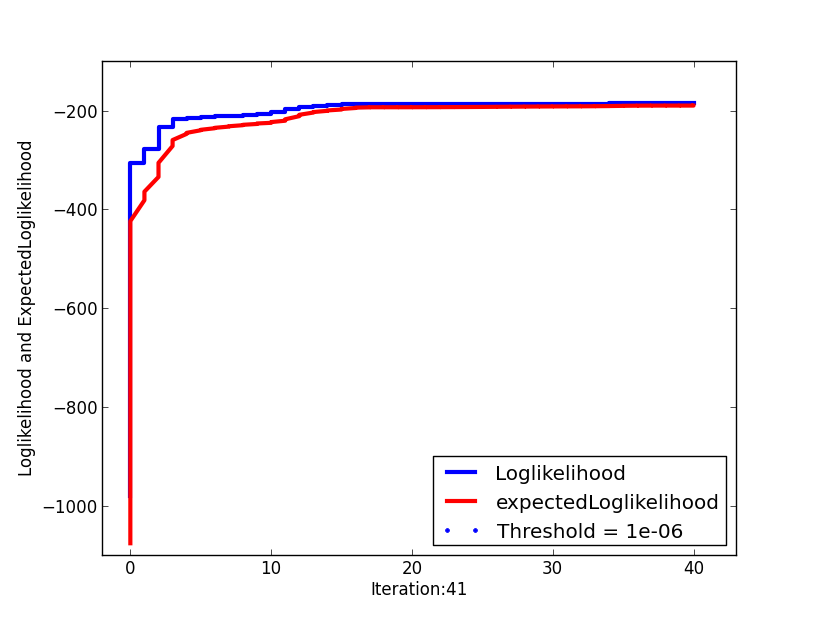
\includegraphics[width=5in,height=3.8in]{./picture/figure_1.png}
\end{center}
(c) Discuss the ratio of the two eigenvalues found with respect to the task of classifying the data in the projected 2-dimensional space. \\
\htab Again, present the the two eigenvalues found first,
    $$ \lambda_{1} = 32.1919292,  \lambda_{2} = 0.285391043 $$
\htab And the ratio of those two eigenvalues are as follows,
    $$ r = \frac{\lambda_{1}}{\lambda_{2}} = 112.799367851 $$
    \htab Note that the horizontal coordinate axis $X_{1}$ corresponds to the dimension with $\lambda_{1}$, the vertical coordinate axis $X_{2}$ corresponds to the dimension with $\lambda_{2}$. \\
    \htab From the result of data projection in two dimension, we can see that \textbf{those three classes has tremendous distinction in the horizental coordinate} (with large eigenvalue), while the differences in the vertical coordinate (with the smaller eigenvalue). Therefore, I believe in the intuition that \textbf{the ratio of two eigenvalues $r$ shows the relative distinguishability (between two dimensions) of data objects from each other class}. And by the way, such distinguisability may come from the large between-class variance and small within-class variance.
\newpage
%}}}
% 3.1.3
%{{{
% 3.1.3
\subsubsection{Codes to Compute criteria $J$}
\htab We have accomplished the codes to compute $S_{w}$, $S_{B}$ and then criteria $J$ for projecting original data into $\V_{1}$ $\V_{2}$, please see getSolution\_3\_3\_, \\
\htab Within-Class Scatter Matrix:\\
$$ S_{W} = \begin{pmatrix}   
    9.31175619 &  -2.18194354\times 10^{-08} \\
    -2.18194354\times 10^{-08}   &  10.7967585  
 \end{pmatrix} $$
\htab Between-Class Scatter Matrix:\\
$$ S_{B} = \begin{pmatrix}
    299.763396  & 2.58546748\times 10^{-06}  \\
    2.58546748\times 10^{-6}  &  3.08129816  
\end{pmatrix} $$
\htab Then, we derive: \\
$$ S_{W}^{-1} S_{B} = \begin{pmatrix}
    32.1919292  &  2.78325001\times 10^{-07} \\
    3.04524474\times 10^{-07}   & 0.285391043
    \end{pmatrix} $$
\htab Finally, we have trace of $ S_{W}^{-1} S_{B} $,
$$ J = tr\{S_{W}^{-1}S_{B}\} = 32.4773202409 $$
%}}}
% 3.1.4
%{{{
\subsubsection{Compare to other projection}
\htab We have achieved automatically derive all combinations of two-axes projection. And use the predefined framework to work out criteria $J$ for each combination, please see getSolution\_3\_4\_, \\ 
\begin{center}
\begin{tabular} {|| c | c ||}
    \hline 
    projecting combo & criteria $J$ \\ \hline 
    $\V_{1}$, $\V_{2}$ & 32.4773202409 \\ \hline 
    Sepal Length ,  Sepal Width  & 4.3327944087 \\ \hline 
    Sepal Length ,  Petal Length  & 23.3646503713 \\ \hline 
    Sepal Length ,  Petal Width  & 13.0644017179 \\ \hline 
    Sepal Width ,  Petal Length  & 21.8610096544 \\ \hline 
    Sepal Width ,  Petal Width  & 20.3468961554 \\ \hline 
    Petal Length ,  Petal Width  & 19.7820503322 \\ \hline 
\end{tabular}
\end{center}
\htab Note that the Sepal Length,  Sepal Width, Petal Length, Petal Width are the 1st, 2nd, 3rd, 4th feature in the original input Iris data, respectively. \\
\htab It is obvious that \textbf{ the practice of projecting data into $\V_{1}$,$\V_{2}$ derived from fisher algorithm has the best outcome in maximizing between-class variance the and minimizing the within-class variance in the meanwhile}, comparing to projecting into any combination of 2-dimensional axes in original space. \\
\htab It may be generalized to a wider conclusion that for any dimension $D' (D'< n)$ ($n$ is the number of input features),  the projecting matrix $W_{n\times D'}$ figured out by fisher's algorithm are the best projection to classify data objects among all possible $D'$-dimension projection. This is for the reason that the indicator $J$ of projection from fisher algorithm's would be largest among all $D'$-dimension projections.
\newpage
%}}}

% 4
\section{Cross Validation and Classification}
% 4.1
\subsection{K-Nearest Neighbours Algorithm}
% 4.1.1 - 4.1.3
%{{{
% 4.1.1
\subsubsection{Implement K-NN algorithm}
\htab See the code file "KNN.py" for implementing the K-NN algorithm. \\
\htab In the KNN.py, the function getSolution\_4\_1\_1 is a test function for the KNN Implementation. It uses the last data object of Iris datasets as the only testing data object and the rest as training dataset. 
\htab I also implement the min-max scaling to the original data since the KNN classifier is \textbf{vulnerable to bad scaling}. (see the scaling function in KNN.py) Specifically, preprocessing towards data, called min-max scaling, is to project each dimension of input $x$ into the range of $[0,1]$,
\begin{equation}
    x := \frac{x - x_{min}}{x_{max} - x_{min}}
\end{equation}
% 4.1.2
\subsubsection{Apply Cross Validation}
\htab Here we provide result of cross validation for scaled input and original input. You can see both results by switching corresponding argument of all "getSolution" functions. \\
\htab Note that the result reported in the following is derived not through shuffling the original input. Because Unshuffled grouping is one particular shuffled grouping in cross validation, I did not implement the shuffling in my code. (in fact, only several lines of codes calling numpy.random is sufficient to achieve that functionality)\\
% unscaled data result
\textbf{For original input data:} \\
\htab For 2-fold cross validation, we pick up $ k = 8 $, 
whose average cross validation test error is $ 4.0 \% $ . 
\hyperlink{twoFoldResultunNorm}{See the tabular result of unscaled 2-fold Cross Validation}. \\
\htab For 5-fold cross validation, we pick up $ k = 12 $, 
whose average cross validation test error is $ 2.0 \% $ . 
\hyperlink{fiveFoldResultunNorm}{See the tabular result of unscaled 5-fold Cross Validation}. \\
\htab For 10-fold cross validation, we pick up $ k = 20 $, 
whose average cross validation test error is $ 2.0 \% $ . 
\hyperlink{tenFoldResultunNorm}{See the tabular result of unscaled 10-fold Cross Validation}. \\[0.5cm]
% scaled data result
\textbf{For scaled input data:} \\
\htab For 2-fold cross validation, we pick up $ k = 11 $, 
whose average cross validation test error is $ 2.67 \% $ . 
\hyperlink{twoFoldResultNorm}{See the tabular result of scaled 2-fold Cross Validation}. \\
\htab For 5-fold cross validation, we pick up $ k = 16 $, 
whose average cross validation test error is $ 2.67 \% $ . 
\hyperlink{fiveFoldResultNorm}{See the tabular result of scaled 5-fold Cross Validation}. \\
\htab For 10-fold cross validation, we pick up $ k = 30 $, 
whose average cross validation test error is $ 2.67 \% $. 
\hyperlink{tenFoldResultNorm}{See the tabular result of scaled 10-fold Cross Validation}. \\[0.5cm]
% reason
\textbf{Why choose larger $k$ if several $k$ has the same lowest error rate:} \\
\htab Under the circumstance that increasing $k$ will not lead to rise of error rate (since the same lowest error we have observed in the experiment), we can use higher value of $k$ to enhance the robustness of classifier. If more nearest neighbours are considered for majority voting without decreasing the error rate, we can determine the result of classification from a larger amount of information (neighbours) by using a greater $k$.

% 4.1.3
\subsubsection{Report result of cross validation}
Considering the beautification of the type setting, the report of cross validation for various $k = 2,4,..,40$ was put in the appendix. \\ 
\htab \hyperlink{kResultUNSCALED}{See report of various $k$ with ORIGINAL data}. \\
\htab \hyperlink{kResultSCALED}{See report of various $k$ with SCALED data}.\\
\newpage
%}}}
% 4.1.4 - 4.1.6
%{{{
% 4.1.4
\subsubsection{Explain optimal error decreases with fold number}
\htab First, let us analyze the source of the error in KNN algorithm. The overall relationship of error and $k$ could be represented by the the first graph below. In the first stage (before it comes to the optima) when $k$ is small, inprecision of decision regions mainly comes from the reason that very few neighbours are considered while classifying a testing data object. Error will be arised in those ambiguous regions like the green testing data obejct in second figure). \\
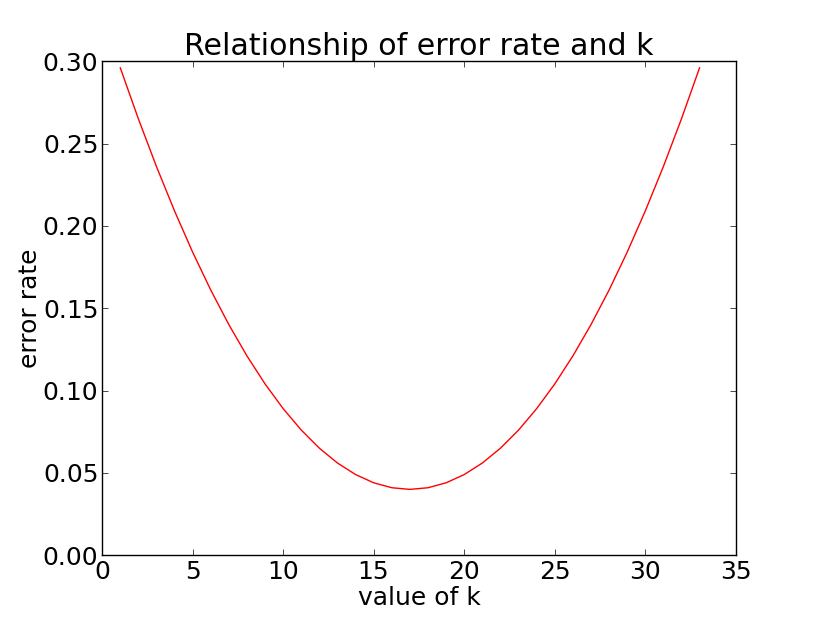
\includegraphics[width=2.2in,height=1.5in]{./picture/F0.png}
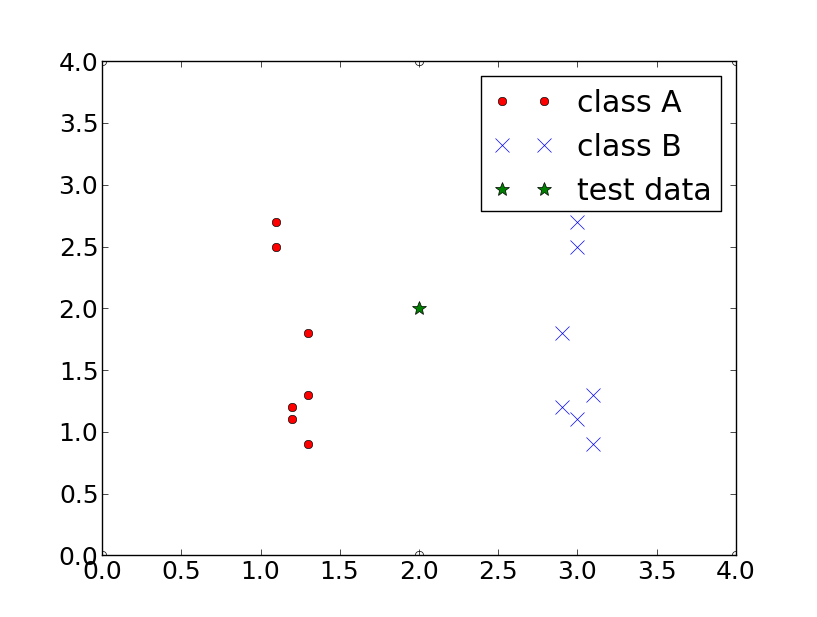
\includegraphics[width=2.2in,height=1.5in]{./picture/F1.png}
\includegraphics[width=2.2in,height=1.5in]{./picture/F2.png}\\
\htab As the fold number rises, \textbf{the number of data objects as training data also increases}. (In the case of Iris-dataset, 2-fold has 75 objects; 5-fold has 120 objects; 10-fold has 135 objects). Since more data objects are used in KNN algorithm, which use training data (rather than a parametric model) as classifier, prediction of testing data object in ambiguous region will be more deterministic and the bias will be effectively decreased. Hence, accuracy of KNN classifier will be enhanced (at least non-decreased). And correspondingly, the optimal errors will decrease with the fold number.
% 4.1.5
\subsubsection{Explain optimal $k$ decreases with fold number}
\htab However, in the second stage when $k$ is large, the error of algorithm is mainly coming from the reason that too many neighbours are considered. See the first image below where the classification of middle testing data is not desirable when $k=10$. 
\begin{center}
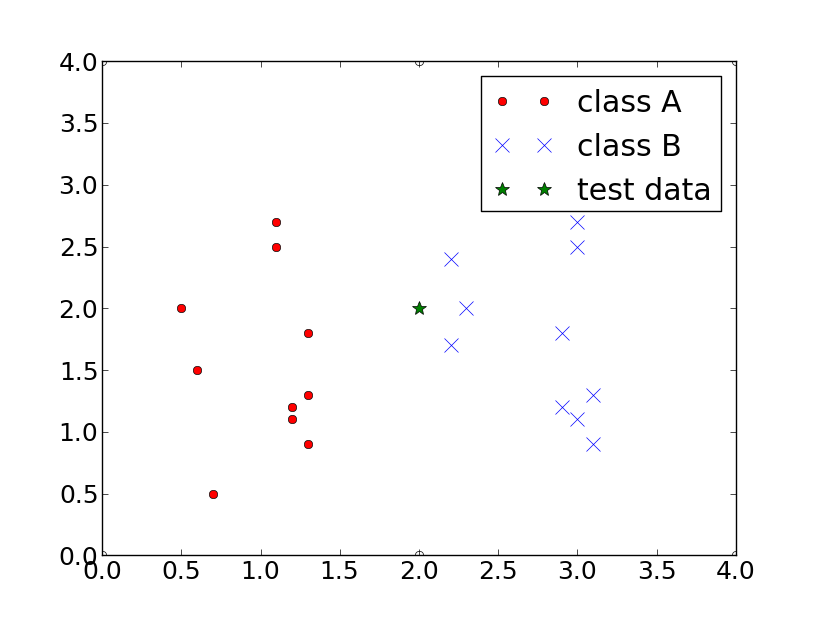
\includegraphics[width=3in,height=2in]{./picture/F3.png}
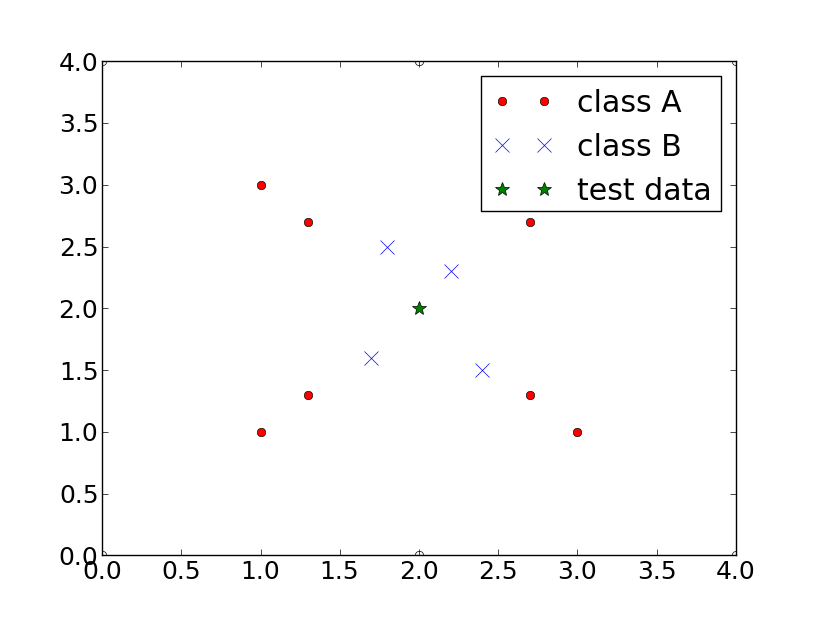
\includegraphics[width=3in,height=2in]{./picture/F4.png}\\
\end{center}
\htab But if more training data objects are given (casued by the increase of fold number), as shown in the second graph, the $k$ must be large enough to make the same classification mistake as in the first case. Here, only when $k=18$, the green test data will be mistaken as of class A. It is concluded from the comparison between two cases above that, \textbf{more training data (or equivalently, higher fold number) in KNN tolerate larger $k$ for optimal error.} Geometrically, the minima would shift considerably rightwards if fold number increase and thereby more training data are used.
\newpage
% 4.1.6
\subsubsection{Listing of programs and solutions}
\begin{verbatim}
KNN.py
    class
        KNNClassifier
        CrossValidation

    member
        __init__ [KNNClassifier]
        getFeatureVector [KNNClassifier]
        getLabel [KNNClassifier]
        getEuclidianDistance [KNNClassifier]
        getDistance [KNNClassifier]
        getKNearestNeighbours [KNNClassifier]
        majorityVoting [KNNClassifier]
        run [KNNClassifier]

        __init__ [CrossValidation]
        getRandomGroup [CrossValidation]
        getError [CrossValidation]
        run [CrossValidation]

    function
        printMatrix
        classMapping
        readMatrix
        scaling
        getSolution_4_1_1_
        getSolution_4_1_2_
        getSolution_4_1_3_
        main
\end{verbatim}
\newpage
%}}}

% appendix
\appendix
% A. proof 
%{{{
\section{Supplementary proof}
\hypertarget{Linearity}{}
\subsection{Proof of linearity of $E(x+y)$ }
\htab Based on definition of expectation, we have
    $$ E(x+y) = \dinfint (x+y) P(x,y) dx dy \eqno (1) $$
    $$ E(x) = \infint x P(x) dx \eqno (2) $$
    $$ E(y) = \infint y P(y) dy \eqno (3) $$
\htab Note that we use $\mu$ as abbreviation of expectation of certain random variable. \\
\htab Then we start manipulating $E(x+y)$ from $(1)$
$$ 
\begin{aligned}
    E(x+y) & = \dinfint \Big[ xP(x,y) + yP(x,y) \Big] dx dy \\
    & = \dinfint xP(x,y) dx dy + \dinfint yP(x,y) dx dy \\
    & = \infint xP(x) dx + \infint yP(y) dy 
\end{aligned}
\eqno (4) $$
\htab Note that last derivation above is based on sum rule of probability. \\
\htab By taking $(2)$ and $(3)$ for $(4)$, we solve the proof
    $$ E(x+y)= E(x) + E(y) \eqno (5) $$
\newpage

\newpage
%}}}

% B. result for Cross validation
\section{Result for Cross Validation}
\subsection{Cross Validation for KNN with ORIGINAL input}
\hypertarget{twoFoldResultunNorm}{}
%{{{
\subsubsection{2-fold}
\begin{center}
    \begin{tabular} {|| c | c | c ||}
        \hline
        item name & average error & error of each group \\ \hline
        2-NN 2-fold CV & 8.00\% & ( 8.00\%, 8.00\% )\\ \hline
        3-NN 2-fold CV & 6.00\% & ( 4.00\%, 8.00\% )\\ \hline
        4-NN 2-fold CV & 4.67\% & ( 4.00\%, 5.33\% )\\ \hline
        5-NN 2-fold CV & 6.00\% & ( 4.00\%, 8.00\% )\\ \hline
        6-NN 2-fold CV & 5.33\% & ( 2.67\%, 8.00\% )\\ \hline
        7-NN 2-fold CV & 6.00\% & ( 5.33\%, 6.67\% )\\ \hline
        8-NN 2-fold CV & 4.00\% & ( 2.67\%, 5.33\% )\\ \hline
        9-NN 2-fold CV & 4.67\% & ( 4.00\%, 5.33\% )\\ \hline
        10-NN 2-fold CV & 4.67\% & ( 2.67\%, 6.67\% )\\ \hline
        11-NN 2-fold CV & 6.00\% & ( 5.33\%, 6.67\% )\\ \hline
        12-NN 2-fold CV & 6.00\% & ( 5.33\%, 6.67\% )\\ \hline
        13-NN 2-fold CV & 6.00\% & ( 6.67\%, 5.33\% )\\ \hline
        14-NN 2-fold CV & 6.00\% & ( 5.33\%, 6.67\% )\\ \hline
        15-NN 2-fold CV & 6.67\% & ( 6.67\%, 6.67\% )\\ \hline
        16-NN 2-fold CV & 6.00\% & ( 6.67\%, 5.33\% )\\ \hline
        17-NN 2-fold CV & 5.33\% & ( 6.67\%, 4.00\% )\\ \hline
        18-NN 2-fold CV & 4.67\% & ( 5.33\%, 4.00\% )\\ \hline
        19-NN 2-fold CV & 6.00\% & ( 6.67\%, 5.33\% )\\ \hline
        20-NN 2-fold CV & 6.00\% & ( 6.67\%, 5.33\% )\\ \hline
        21-NN 2-fold CV & 6.00\% & ( 6.67\%, 5.33\% )\\ \hline
        22-NN 2-fold CV & 6.67\% & ( 5.33\%, 8.00\% )\\ \hline
        23-NN 2-fold CV & 5.33\% & ( 5.33\%, 5.33\% )\\ \hline
        24-NN 2-fold CV & 5.33\% & ( 5.33\%, 5.33\% )\\ \hline
        25-NN 2-fold CV & 6.00\% & ( 5.33\%, 6.67\% )\\ \hline
        26-NN 2-fold CV & 7.33\% & ( 6.67\%, 8.00\% )\\ \hline
        27-NN 2-fold CV & 7.33\% & ( 6.67\%, 8.00\% )\\ \hline
        28-NN 2-fold CV & 8.00\% & ( 8.00\%, 8.00\% )\\ \hline
        29-NN 2-fold CV & 8.67\% & ( 8.00\%, 9.33\% )\\ \hline
        30-NN 2-fold CV & 9.33\% & ( 9.33\%, 9.33\% )\\ \hline
        31-NN 2-fold CV & 9.33\% & ( 9.33\%, 9.33\% )\\ \hline
        32-NN 2-fold CV & 9.33\% & ( 9.33\%, 9.33\% )\\ \hline
        33-NN 2-fold CV & 10.00\% & ( 9.33\%, 10.67\% )\\ \hline
        34-NN 2-fold CV & 9.33\% & ( 9.33\%, 9.33\% )\\ \hline
        35-NN 2-fold CV & 8.67\% & ( 8.00\%, 9.33\% )\\ \hline
        36-NN 2-fold CV & 10.67\% & ( 10.67\%, 10.67\% )\\ \hline
        37-NN 2-fold CV & 10.67\% & ( 10.67\%, 10.67\% )\\ \hline
        38-NN 2-fold CV & 11.33\% & ( 10.67\%, 12.00\% )\\ \hline
        39-NN 2-fold CV & 11.33\% & ( 10.67\%, 12.00\% )\\ \hline
\end{tabular}
\end{center}
\newpage
%}}}

\hypertarget{fiveFoldResultunNorm}{}
%{{{
\subsubsection{5-fold}
\begin{center}
    \begin{tabular} {|| c | c | c ||}
        \hline
        item name & average error & error of each group \\ \hline
        2-NN 5-fold CV & 5.33\% & ( 3.33\%, 6.67\%, 6.67\%, 10.00\%, 0.00\% )\\ \hline
        3-NN 5-fold CV & 3.33\% & ( 3.33\%, 3.33\%, 6.67\%, 3.33\%, 0.00\% )\\ \hline
        4-NN 5-fold CV & 2.67\% & ( 3.33\%, 3.33\%, 3.33\%, 3.33\%, 0.00\% )\\ \hline
        5-NN 5-fold CV & 2.67\% & ( 3.33\%, 0.00\%, 6.67\%, 3.33\%, 0.00\% )\\ \hline
        6-NN 5-fold CV & 2.00\% & ( 3.33\%, 0.00\%, 3.33\%, 3.33\%, 0.00\% )\\ \hline
        7-NN 5-fold CV & 2.00\% & ( 3.33\%, 0.00\%, 3.33\%, 3.33\%, 0.00\% )\\ \hline
        8-NN 5-fold CV & 3.33\% & ( 3.33\%, 0.00\%, 6.67\%, 6.67\%, 0.00\% )\\ \hline
        9-NN 5-fold CV & 2.67\% & ( 3.33\%, 0.00\%, 3.33\%, 6.67\%, 0.00\% )\\ \hline
        10-NN 5-fold CV & 2.00\% & ( 3.33\%, 0.00\%, 0.00\%, 6.67\%, 0.00\% )\\ \hline
        11-NN 5-fold CV & 2.00\% & ( 6.67\%, 0.00\%, 0.00\%, 3.33\%, 0.00\% )\\ \hline
        12-NN 5-fold CV & 2.00\% & ( 6.67\%, 0.00\%, 0.00\%, 3.33\%, 0.00\% )\\ \hline
        13-NN 5-fold CV & 2.67\% & ( 6.67\%, 0.00\%, 3.33\%, 3.33\%, 0.00\% )\\ \hline
        14-NN 5-fold CV & 3.33\% & ( 6.67\%, 0.00\%, 3.33\%, 6.67\%, 0.00\% )\\ \hline
        15-NN 5-fold CV & 3.33\% & ( 6.67\%, 0.00\%, 6.67\%, 3.33\%, 0.00\% )\\ \hline
        16-NN 5-fold CV & 3.33\% & ( 6.67\%, 0.00\%, 6.67\%, 3.33\%, 0.00\% )\\ \hline
        17-NN 5-fold CV & 3.33\% & ( 6.67\%, 0.00\%, 6.67\%, 3.33\%, 0.00\% )\\ \hline
        18-NN 5-fold CV & 2.67\% & ( 6.67\%, 0.00\%, 3.33\%, 3.33\%, 0.00\% )\\ \hline
        19-NN 5-fold CV & 3.33\% & ( 6.67\%, 0.00\%, 6.67\%, 3.33\%, 0.00\% )\\ \hline
        20-NN 5-fold CV & 4.00\% & ( 6.67\%, 0.00\%, 6.67\%, 6.67\%, 0.00\% )\\ \hline
        21-NN 5-fold CV & 3.33\% & ( 6.67\%, 0.00\%, 6.67\%, 3.33\%, 0.00\% )\\ \hline
        22-NN 5-fold CV & 4.00\% & ( 6.67\%, 0.00\%, 6.67\%, 6.67\%, 0.00\% )\\ \hline
        23-NN 5-fold CV & 4.00\% & ( 6.67\%, 0.00\%, 6.67\%, 6.67\%, 0.00\% )\\ \hline
        24-NN 5-fold CV & 5.33\% & ( 6.67\%, 3.33\%, 10.00\%, 6.67\%, 0.00\% )\\ \hline
        25-NN 5-fold CV & 4.67\% & ( 10.00\%, 3.33\%, 6.67\%, 3.33\%, 0.00\% )\\ \hline
        26-NN 5-fold CV & 5.33\% & ( 10.00\%, 3.33\%, 6.67\%, 6.67\%, 0.00\% )\\ \hline
        27-NN 5-fold CV & 5.33\% & ( 10.00\%, 3.33\%, 6.67\%, 6.67\%, 0.00\% )\\ \hline
        28-NN 5-fold CV & 5.33\% & ( 10.00\%, 3.33\%, 6.67\%, 6.67\%, 0.00\% )\\ \hline
        29-NN 5-fold CV & 6.00\% & ( 10.00\%, 3.33\%, 10.00\%, 6.67\%, 0.00\% )\\ \hline
        30-NN 5-fold CV & 6.00\% & ( 10.00\%, 3.33\%, 6.67\%, 10.00\%, 0.00\% )\\ \hline
        31-NN 5-fold CV & 6.00\% & ( 10.00\%, 3.33\%, 10.00\%, 6.67\%, 0.00\% )\\ \hline
        32-NN 5-fold CV & 6.00\% & ( 10.00\%, 3.33\%, 6.67\%, 10.00\%, 0.00\% )\\ \hline
        33-NN 5-fold CV & 6.67\% & ( 10.00\%, 3.33\%, 10.00\%, 10.00\%, 0.00\% )\\ \hline
        34-NN 5-fold CV & 4.67\% & ( 6.67\%, 3.33\%, 6.67\%, 6.67\%, 0.00\% )\\ \hline
        35-NN 5-fold CV & 5.33\% & ( 10.00\%, 3.33\%, 6.67\%, 6.67\%, 0.00\% )\\ \hline
        36-NN 5-fold CV & 5.33\% & ( 10.00\%, 3.33\%, 6.67\%, 6.67\%, 0.00\% )\\ \hline
        37-NN 5-fold CV & 5.33\% & ( 10.00\%, 3.33\%, 6.67\%, 6.67\%, 0.00\% )\\ \hline
        38-NN 5-fold CV & 7.33\% & ( 10.00\%, 6.67\%, 13.33\%, 6.67\%, 0.00\% )\\ \hline
39-NN 5-fold CV & 5.33\% & ( 10.00\%, 6.67\%, 6.67\%, 3.33\%, 0.00\% )\\ \hline
    \end{tabular}
\end{center}
\newpage
%}}}

\hypertarget{tenFoldResultunNorm}{}
%{{{
\subsubsection{10-fold}
\begin{center}
    \begin{tabular} {|| c | c | c ||}
        \hline
        item  & AVG & error of each group \\ \hline
2-NN & 4.67\% & ( 0.00\%, 6.67\%, 0.00\%, 6.67\%, 13.33\%, 0.00\%, 13.33\%, 6.67\%, 0.00\%, 0.00\% )\\ \hline
3-NN & 3.33\% & ( 0.00\%, 6.67\%, 0.00\%, 6.67\%, 13.33\%, 0.00\%, 6.67\%, 0.00\%, 0.00\%, 0.00\% )\\ \hline
4-NN & 3.33\% & ( 0.00\%, 6.67\%, 0.00\%, 6.67\%, 13.33\%, 0.00\%, 6.67\%, 0.00\%, 0.00\%, 0.00\% )\\ \hline
5-NN & 3.33\% & ( 0.00\%, 6.67\%, 0.00\%, 0.00\%, 13.33\%, 6.67\%, 6.67\%, 0.00\%, 0.00\%, 0.00\% )\\ \hline
6-NN & 3.33\% & ( 0.00\%, 6.67\%, 0.00\%, 0.00\%, 13.33\%, 6.67\%, 6.67\%, 0.00\%, 0.00\%, 0.00\% )\\ \hline
7-NN & 3.33\% & ( 0.00\%, 6.67\%, 0.00\%, 0.00\%, 13.33\%, 6.67\%, 6.67\%, 0.00\%, 0.00\%, 0.00\% )\\ \hline
8-NN & 3.33\% & ( 0.00\%, 6.67\%, 0.00\%, 0.00\%, 0.00\%, 13.33\%, 6.67\%, 6.67\%, 0.00\%, 0.00\% )\\ \hline
9-NN & 2.67\% & ( 0.00\%, 6.67\%, 0.00\%, 0.00\%, 0.00\%, 6.67\%, 6.67\%, 6.67\%, 0.00\%, 0.00\% )\\ \hline
10-NN & 3.33\% & ( 0.00\%, 6.67\%, 0.00\%, 0.00\%, 0.00\%, 13.33\%, 6.67\%, 6.67\%, 0.00\%, 0.00\% )\\ \hline
11-NN & 3.33\% & ( 0.00\%, 6.67\%, 0.00\%, 0.00\%, 0.00\%, 13.33\%, 6.67\%, 6.67\%, 0.00\%, 0.00\% )\\ \hline
12-NN & 2.67\% & ( 0.00\%, 6.67\%, 0.00\%, 0.00\%, 0.00\%, 6.67\%, 6.67\%, 6.67\%, 0.00\%, 0.00\% )\\ \hline
13-NN & 2.00\% & ( 0.00\%, 6.67\%, 0.00\%, 0.00\%, 0.00\%, 6.67\%, 6.67\%, 0.00\%, 0.00\%, 0.00\% )\\ \hline
14-NN & 2.67\% & ( 0.00\%, 6.67\%, 0.00\%, 0.00\%, 0.00\%, 13.33\%, 6.67\%, 0.00\%, 0.00\%, 0.00\% )\\ \hline
15-NN & 2.67\% & ( 6.67\%, 6.67\%, 0.00\%, 0.00\%, 0.00\%, 6.67\%, 6.67\%, 0.00\%, 0.00\%, 0.00\% )\\ \hline
16-NN & 2.67\% & ( 0.00\%, 6.67\%, 0.00\%, 0.00\%, 0.00\%, 6.67\%, 6.67\%, 6.67\%, 0.00\%, 0.00\% )\\ \hline
17-NN & 2.67\% & ( 6.67\%, 6.67\%, 0.00\%, 0.00\%, 0.00\%, 6.67\%, 6.67\%, 0.00\%, 0.00\%, 0.00\% )\\ \hline
18-NN & 2.00\% & ( 0.00\%, 6.67\%, 0.00\%, 0.00\%, 0.00\%, 6.67\%, 6.67\%, 0.00\%, 0.00\%, 0.00\% )\\ \hline
19-NN & 2.67\% & ( 6.67\%, 6.67\%, 0.00\%, 0.00\%, 0.00\%, 6.67\%, 6.67\%, 0.00\%, 0.00\%, 0.00\% )\\ \hline
20-NN & 2.00\% & ( 0.00\%, 6.67\%, 0.00\%, 0.00\%, 0.00\%, 6.67\%, 6.67\%, 0.00\%, 0.00\%, 0.00\% )\\ \hline
21-NN & 3.33\% & ( 6.67\%, 6.67\%, 0.00\%, 0.00\%, 6.67\%, 6.67\%, 6.67\%, 0.00\%, 0.00\%, 0.00\% )\\ \hline
22-NN & 3.33\% & ( 6.67\%, 6.67\%, 0.00\%, 0.00\%, 0.00\%, 6.67\%, 6.67\%, 6.67\%, 0.00\%, 0.00\% )\\ \hline
23-NN & 2.67\% & ( 6.67\%, 6.67\%, 0.00\%, 0.00\%, 0.00\%, 6.67\%, 6.67\%, 0.00\%, 0.00\%, 0.00\% )\\ \hline
24-NN & 4.00\% & ( 6.67\%, 6.67\%, 0.00\%, 0.00\%, 0.00\%, 13.33\%, 6.67\%, 6.67\%, 0.00\%, 0.00\% )\\ \hline
25-NN & 3.33\% & ( 6.67\%, 6.67\%, 0.00\%, 0.00\%, 0.00\%, 6.67\%, 6.67\%, 6.67\%, 0.00\%, 0.00\% )\\ \hline
26-NN & 4.00\% & ( 6.67\%, 6.67\%, 0.00\%, 0.00\%, 0.00\%, 13.33\%, 6.67\%, 6.67\%, 0.00\%, 0.00\% )\\ \hline
27-NN & 3.33\% & ( 6.67\%, 6.67\%, 0.00\%, 0.00\%, 0.00\%, 13.33\%, 6.67\%, 0.00\%, 0.00\%, 0.00\% )\\ \hline
28-NN & 4.67\% & ( 6.67\%, 6.67\%, 0.00\%, 6.67\%, 0.00\%, 13.33\%, 6.67\%, 6.67\%, 0.00\%, 0.00\% )\\ \hline
29-NN & 5.33\% & ( 13.33\%, 6.67\%, 0.00\%, 6.67\%, 0.00\%, 13.33\%, 6.67\%, 6.67\%, 0.00\%, 0.00\% )\\ \hline
30-NN & 5.33\% & ( 13.33\%, 6.67\%, 0.00\%, 6.67\%, 0.00\%, 13.33\%, 6.67\%, 6.67\%, 0.00\%, 0.00\% )\\ \hline
31-NN & 5.33\% & ( 13.33\%, 6.67\%, 0.00\%, 6.67\%, 0.00\%, 13.33\%, 6.67\%, 6.67\%, 0.00\%, 0.00\% )\\ \hline
32-NN & 5.33\% & ( 13.33\%, 6.67\%, 0.00\%, 6.67\%, 0.00\%, 13.33\%, 6.67\%, 6.67\%, 0.00\%, 0.00\% )\\ \hline
33-NN & 5.33\% & ( 13.33\%, 6.67\%, 0.00\%, 6.67\%, 0.00\%, 13.33\%, 6.67\%, 6.67\%, 0.00\%, 0.00\% )\\ \hline
34-NN & 4.67\% & ( 6.67\%, 6.67\%, 0.00\%, 6.67\%, 0.00\%, 13.33\%, 6.67\%, 6.67\%, 0.00\%, 0.00\% )\\ \hline
35-NN & 4.67\% & ( 6.67\%, 6.67\%, 0.00\%, 6.67\%, 0.00\%, 13.33\%, 6.67\%, 6.67\%, 0.00\%, 0.00\% )\\ \hline
36-NN & 5.33\% & ( 6.67\%, 6.67\%, 0.00\%, 6.67\%, 0.00\%, 13.33\%, 13.33\%, 6.67\%, 0.00\%, 0.00\% )\\ \hline
37-NN & 5.33\% & ( 6.67\%, 6.67\%, 0.00\%, 6.67\%, 0.00\%, 13.33\%, 13.33\%, 6.67\%, 0.00\%, 0.00\% )\\ \hline
38-NN & 5.33\% & ( 6.67\%, 6.67\%, 0.00\%, 6.67\%, 0.00\%, 20.00\%, 6.67\%, 6.67\%, 0.00\%, 0.00\% )\\ \hline
39-NN & 5.33\% & ( 13.33\%, 6.67\%, 0.00\%, 6.67\%, 0.00\%, 13.33\%, 6.67\%, 6.67\%, 0.00\%, 0.00\% )\\ \hline
    \end{tabular}
\end{center}
\newpage
%}}}

\subsection{Cross Validation for KNN with SCALED input}
\hypertarget{twoFoldResultNorm}{}
%{{{
\subsubsection{2-fold}
\begin{center}
    \begin{tabular} {|| c | c | c ||}
        \hline
        item name & average error & error of each group \\ \hline
       2NN 2-fold CV & 6.00\% & ( 4.00\%, 8.00\% ) \\ \hline
        3NN 2-fold CV & 4.67\% & ( 5.33\%, 4.00\% ) \\ \hline
        4NN 2-fold CV & 3.33\% & ( 4.00\%, 2.67\% ) \\ \hline
        5NN 2-fold CV & 4.67\% & ( 4.00\%, 5.33\% ) \\ \hline
        6NN 2-fold CV & 4.67\% & ( 5.33\%, 4.00\% ) \\ \hline
        7NN 2-fold CV & 4.67\% & ( 5.33\%, 4.00\% ) \\ \hline
        8NN 2-fold CV & 4.00\% & ( 4.00\%, 4.00\% ) \\ \hline
        9NN 2-fold CV & 4.67\% & ( 4.00\%, 5.33\% ) \\ \hline
        10NN 2-fold CV & 4.00\% & ( 4.00\%, 4.00\% ) \\ \hline
        11NN 2-fold CV & 2.67\% & ( 4.00\%, 1.33\% ) \\ \hline
        12NN 2-fold CV & 3.33\% & ( 4.00\%, 2.67\% ) \\ \hline
        13NN 2-fold CV & 4.00\% & ( 5.33\%, 2.67\% ) \\ \hline
        14NN 2-fold CV & 5.33\% & ( 5.33\%, 5.33\% ) \\ \hline
        15NN 2-fold CV & 4.67\% & ( 5.33\%, 4.00\% ) \\ \hline
        16NN 2-fold CV & 6.67\% & ( 5.33\%, 8.00\% ) \\ \hline
        17NN 2-fold CV & 6.67\% & ( 6.67\%, 6.67\% ) \\ \hline
        18NN 2-fold CV & 4.67\% & ( 2.67\%, 6.67\% ) \\ \hline
        19NN 2-fold CV & 5.33\% & ( 5.33\%, 5.33\% ) \\ \hline
        20NN 2-fold CV & 5.33\% & ( 5.33\%, 5.33\% ) \\ \hline
        21NN 2-fold CV & 5.33\% & ( 5.33\%, 5.33\% ) \\ \hline
        22NN 2-fold CV & 6.00\% & ( 5.33\%, 6.67\% ) \\ \hline
        23NN 2-fold CV & 6.00\% & ( 5.33\%, 6.67\% ) \\ \hline
        24NN 2-fold CV & 6.67\% & ( 5.33\%, 8.00\% ) \\ \hline
        25NN 2-fold CV & 6.67\% & ( 5.33\%, 8.00\% ) \\ \hline
        26NN 2-fold CV & 8.00\% & ( 8.00\%, 8.00\% ) \\ \hline
        27NN 2-fold CV & 8.67\% & ( 8.00\%, 9.33\% ) \\ \hline
        28NN 2-fold CV & 9.33\% & ( 9.33\%, 9.33\% ) \\ \hline
        29NN 2-fold CV & 9.33\% & ( 10.67\%, 8.00\% ) \\ \hline
        30NN 2-fold CV & 11.33\% & ( 12.00\%, 10.67\% ) \\ \hline
        31NN 2-fold CV & 11.33\% & ( 12.00\%, 10.67\% ) \\ \hline
        32NN 2-fold CV & 11.33\% & ( 12.00\%, 10.67\% ) \\ \hline
        33NN 2-fold CV & 12.00\% & ( 13.33\%, 10.67\% ) \\ \hline
        34NN 2-fold CV & 12.00\% & ( 13.33\%, 10.67\% ) \\ \hline
        35NN 2-fold CV & 12.00\% & ( 13.33\%, 10.67\% ) \\ \hline
        36NN 2-fold CV & 12.00\% & ( 13.33\%, 10.67\% ) \\ \hline
        37NN 2-fold CV & 12.00\% & ( 13.33\%, 10.67\% ) \\ \hline
        38NN 2-fold CV & 12.00\% & ( 12.00\%, 12.00\% ) \\ \hline
        39NN 2-fold CV & 12.67\% & ( 13.33\%, 12.00\% ) \\ \hline 
    \end{tabular}
\end{center}
\newpage
%}}}

\hypertarget{fiveFoldResultNorm}{}
%{{{
\subsubsection{5-fold}
\begin{center}
    \begin{tabular} {|| c | c | c ||}
        \hline
        item name & average error & error of each group \\ \hline
        2NN 5-fold CV & 4.00\% & ( 3.33\%, 3.33\%, 3.33\%, 10.00\%, 0.00\% ) \\ \hline
        3NN 5-fold CV & 4.67\% & ( 3.33\%, 3.33\%, 6.67\%, 10.00\%, 0.00\% ) \\ \hline
        4NN 5-fold CV & 3.33\% & ( 3.33\%, 3.33\%, 0.00\%, 10.00\%, 0.00\% ) \\ \hline
        5NN 5-fold CV & 4.00\% & ( 3.33\%, 3.33\%, 3.33\%, 10.00\%, 0.00\% ) \\ \hline
        6NN 5-fold CV & 3.33\% & ( 3.33\%, 3.33\%, 0.00\%, 10.00\%, 0.00\% ) \\ \hline
        7NN 5-fold CV & 4.00\% & ( 3.33\%, 3.33\%, 3.33\%, 10.00\%, 0.00\% ) \\ \hline
        8NN 5-fold CV & 4.00\% & ( 3.33\%, 3.33\%, 3.33\%, 10.00\%, 0.00\% ) \\ \hline
        9NN 5-fold CV & 4.00\% & ( 3.33\%, 3.33\%, 3.33\%, 10.00\%, 0.00\% ) \\ \hline
        10NN 5-fold CV & 4.00\% & ( 3.33\%, 3.33\%, 3.33\%, 10.00\%, 0.00\% ) \\ \hline
        11NN 5-fold CV & 4.00\% & ( 3.33\%, 3.33\%, 3.33\%, 10.00\%, 0.00\% ) \\ \hline
        12NN 5-fold CV & 4.00\% & ( 3.33\%, 3.33\%, 3.33\%, 10.00\%, 0.00\% ) \\ \hline
        13NN 5-fold CV & 4.00\% & ( 3.33\%, 3.33\%, 3.33\%, 10.00\%, 0.00\% ) \\ \hline
        14NN 5-fold CV & 3.33\% & ( 3.33\%, 3.33\%, 0.00\%, 10.00\%, 0.00\% ) \\ \hline
        15NN 5-fold CV & 2.67\% & ( 3.33\%, 3.33\%, 0.00\%, 6.67\%, 0.00\% ) \\ \hline
        16NN 5-fold CV & 2.67\% & ( 3.33\%, 3.33\%, 0.00\%, 6.67\%, 0.00\% ) \\ \hline
        17NN 5-fold CV & 4.00\% & ( 3.33\%, 3.33\%, 6.67\%, 6.67\%, 0.00\% ) \\ \hline
        18NN 5-fold CV & 3.33\% & ( 3.33\%, 3.33\%, 3.33\%, 6.67\%, 0.00\% ) \\ \hline
        19NN 5-fold CV & 5.33\% & ( 6.67\%, 3.33\%, 6.67\%, 10.00\%, 0.00\% ) \\ \hline
        20NN 5-fold CV & 4.00\% & ( 6.67\%, 3.33\%, 0.00\%, 10.00\%, 0.00\% ) \\ \hline
        21NN 5-fold CV & 5.33\% & ( 6.67\%, 3.33\%, 6.67\%, 10.00\%, 0.00\% ) \\ \hline
        22NN 5-fold CV & 4.67\% & ( 6.67\%, 3.33\%, 3.33\%, 10.00\%, 0.00\% ) \\ \hline
        23NN 5-fold CV & 4.67\% & ( 6.67\%, 3.33\%, 6.67\%, 6.67\%, 0.00\% ) \\ \hline
        24NN 5-fold CV & 4.67\% & ( 6.67\%, 3.33\%, 3.33\%, 10.00\%, 0.00\% ) \\ \hline
        25NN 5-fold CV & 5.33\% & ( 6.67\%, 3.33\%, 6.67\%, 10.00\%, 0.00\% ) \\ \hline
        26NN 5-fold CV & 4.00\% & ( 6.67\%, 3.33\%, 3.33\%, 6.67\%, 0.00\% ) \\ \hline
        27NN 5-fold CV & 4.00\% & ( 6.67\%, 3.33\%, 3.33\%, 6.67\%, 0.00\% ) \\ \hline
        28NN 5-fold CV & 4.00\% & ( 6.67\%, 3.33\%, 3.33\%, 6.67\%, 0.00\% ) \\ \hline
        29NN 5-fold CV & 4.00\% & ( 6.67\%, 3.33\%, 3.33\%, 6.67\%, 0.00\% ) \\ \hline
        30NN 5-fold CV & 4.00\% & ( 3.33\%, 3.33\%, 3.33\%, 10.00\%, 0.00\% ) \\ \hline
        31NN 5-fold CV & 4.00\% & ( 3.33\%, 3.33\%, 3.33\%, 10.00\%, 0.00\% ) \\ \hline
        32NN 5-fold CV & 4.00\% & ( 3.33\%, 3.33\%, 3.33\%, 10.00\%, 0.00\% ) \\ \hline
        33NN 5-fold CV & 4.00\% & ( 3.33\%, 3.33\%, 3.33\%, 10.00\%, 0.00\% ) \\ \hline
        34NN 5-fold CV & 4.00\% & ( 3.33\%, 3.33\%, 3.33\%, 10.00\%, 0.00\% ) \\ \hline
        35NN 5-fold CV & 5.33\% & ( 10.00\%, 3.33\%, 3.33\%, 10.00\%, 0.00\% ) \\ \hline
        36NN 5-fold CV & 5.33\% & ( 10.00\%, 3.33\%, 3.33\%, 10.00\%, 0.00\% ) \\ \hline
        37NN 5-fold CV & 5.33\% & ( 10.00\%, 3.33\%, 3.33\%, 10.00\%, 0.00\% ) \\ \hline
        38NN 5-fold CV & 4.67\% & ( 6.67\%, 3.33\%, 3.33\%, 10.00\%, 0.00\% ) \\ \hline
        39NN 5-fold CV & 4.67\% & ( 6.67\%, 3.33\%, 3.33\%, 10.00\%, 0.00\% ) \\ \hline
    \end{tabular}
\end{center}
\newpage
%}}}

\hypertarget{tenFoldResultNorm}{}
%{{{
\subsubsection{10-fold}
\begin{center}
    \begin{tabular} {|| c | c | c ||}
        \hline
        item  & AVE & error of each group \\ \hline
2NN & 4.00\% & ( 0.00\%, 6.67\%, 0.00\%, 6.67\%, 6.67\%, 0.00\%, 20.00\%, 0.00\%, 0.00\%, 0.00\% ) \\ \hline
3NN & 4.67\% & ( 0.00\%, 6.67\%, 0.00\%, 6.67\%, 13.33\%, 0.00\%, 20.00\%, 0.00\%, 0.00\%, 0.00\% ) \\ \hline
4NN & 4.00\% & ( 0.00\%, 6.67\%, 0.00\%, 6.67\%, 6.67\%, 0.00\%, 20.00\%, 0.00\%, 0.00\%, 0.00\% ) \\ \hline
5NN & 4.67\% & ( 0.00\%, 6.67\%, 0.00\%, 6.67\%, 6.67\%, 6.67\%, 20.00\%, 0.00\%, 0.00\%, 0.00\% ) \\ \hline
6NN & 3.33\% & ( 0.00\%, 6.67\%, 0.00\%, 6.67\%, 0.00\%, 0.00\%, 20.00\%, 0.00\%, 0.00\%, 0.00\% ) \\ \hline
7NN & 4.00\% & ( 0.00\%, 6.67\%, 0.00\%, 6.67\%, 0.00\%, 6.67\%, 20.00\%, 0.00\%, 0.00\%, 0.00\% ) \\ \hline
8NN & 4.00\% & ( 0.00\%, 6.67\%, 0.00\%, 6.67\%, 0.00\%, 6.67\%, 20.00\%, 0.00\%, 0.00\%, 0.00\% ) \\ \hline
9NN & 4.00\% & ( 0.00\%, 6.67\%, 0.00\%, 0.00\%, 6.67\%, 6.67\%, 20.00\%, 0.00\%, 0.00\%, 0.00\% ) \\ \hline
10NN & 4.00\% & ( 0.00\%, 6.67\%, 0.00\%, 6.67\%, 0.00\%, 6.67\%, 20.00\%, 0.00\%, 0.00\%, 0.00\% ) \\ \hline
11NN & 4.67\% & ( 0.00\%, 6.67\%, 0.00\%, 6.67\%, 6.67\%, 6.67\%, 20.00\%, 0.00\%, 0.00\%, 0.00\% ) \\ \hline
12NN & 4.00\% & ( 0.00\%, 6.67\%, 0.00\%, 6.67\%, 0.00\%, 6.67\%, 20.00\%, 0.00\%, 0.00\%, 0.00\% ) \\ \hline
13NN & 4.00\% & ( 0.00\%, 6.67\%, 0.00\%, 6.67\%, 0.00\%, 6.67\%, 20.00\%, 0.00\%, 0.00\%, 0.00\% ) \\ \hline
14NN & 4.00\% & ( 0.00\%, 6.67\%, 0.00\%, 6.67\%, 0.00\%, 6.67\%, 20.00\%, 0.00\%, 0.00\%, 0.00\% ) \\ \hline
15NN & 3.33\% & ( 0.00\%, 6.67\%, 0.00\%, 6.67\%, 0.00\%, 6.67\%, 13.33\%, 0.00\%, 0.00\%, 0.00\% ) \\ \hline
16NN & 3.33\% & ( 0.00\%, 6.67\%, 0.00\%, 6.67\%, 0.00\%, 0.00\%, 13.33\%, 6.67\%, 0.00\%, 0.00\% ) \\ \hline
17NN & 3.33\% & ( 0.00\%, 6.67\%, 0.00\%, 6.67\%, 0.00\%, 6.67\%, 13.33\%, 0.00\%, 0.00\%, 0.00\% ) \\ \hline
18NN & 4.00\% & ( 0.00\%, 6.67\%, 0.00\%, 6.67\%, 0.00\%, 6.67\%, 20.00\%, 0.00\%, 0.00\%, 0.00\% ) \\ \hline
19NN & 4.67\% & ( 0.00\%, 6.67\%, 0.00\%, 6.67\%, 6.67\%, 6.67\%, 20.00\%, 0.00\%, 0.00\%, 0.00\% ) \\ \hline
20NN & 4.67\% & ( 0.00\%, 6.67\%, 0.00\%, 6.67\%, 6.67\%, 6.67\%, 20.00\%, 0.00\%, 0.00\%, 0.00\% ) \\ \hline
21NN & 4.67\% & ( 0.00\%, 6.67\%, 0.00\%, 6.67\%, 6.67\%, 6.67\%, 20.00\%, 0.00\%, 0.00\%, 0.00\% ) \\ \hline
22NN & 4.00\% & ( 0.00\%, 6.67\%, 0.00\%, 6.67\%, 6.67\%, 0.00\%, 20.00\%, 0.00\%, 0.00\%, 0.00\% ) \\ \hline
23NN & 4.67\% & ( 0.00\%, 6.67\%, 0.00\%, 6.67\%, 6.67\%, 6.67\%, 20.00\%, 0.00\%, 0.00\%, 0.00\% ) \\ \hline
24NN & 3.33\% & ( 0.00\%, 6.67\%, 0.00\%, 6.67\%, 0.00\%, 0.00\%, 20.00\%, 0.00\%, 0.00\%, 0.00\% ) \\ \hline
25NN & 5.33\% & ( 6.67\%, 6.67\%, 0.00\%, 6.67\%, 6.67\%, 6.67\%, 20.00\%, 0.00\%, 0.00\%, 0.00\% ) \\ \hline
26NN & 4.67\% & ( 6.67\%, 6.67\%, 0.00\%, 6.67\%, 6.67\%, 0.00\%, 20.00\%, 0.00\%, 0.00\%, 0.00\% ) \\ \hline
27NN & 5.33\% & ( 6.67\%, 6.67\%, 0.00\%, 6.67\%, 6.67\%, 6.67\%, 20.00\%, 0.00\%, 0.00\%, 0.00\% ) \\ \hline
28NN & 4.00\% & ( 0.00\%, 6.67\%, 0.00\%, 6.67\%, 6.67\%, 0.00\%, 20.00\%, 0.00\%, 0.00\%, 0.00\% ) \\ \hline
29NN & 4.00\% & ( 0.00\%, 6.67\%, 0.00\%, 6.67\%, 6.67\%, 0.00\%, 20.00\%, 0.00\%, 0.00\%, 0.00\% ) \\ \hline
30NN & 2.67\% & ( 0.00\%, 6.67\%, 0.00\%, 6.67\%, 0.00\%, 0.00\%, 13.33\%, 0.00\%, 0.00\%, 0.00\% ) \\ \hline
31NN & 4.00\% & ( 6.67\%, 6.67\%, 0.00\%, 6.67\%, 0.00\%, 6.67\%, 13.33\%, 0.00\%, 0.00\%, 0.00\% ) \\ \hline
32NN & 4.00\% & ( 0.00\%, 6.67\%, 0.00\%, 6.67\%, 0.00\%, 6.67\%, 13.33\%, 6.67\%, 0.00\%, 0.00\% ) \\ \hline
33NN & 4.00\% & ( 0.00\%, 6.67\%, 0.00\%, 6.67\%, 0.00\%, 6.67\%, 13.33\%, 6.67\%, 0.00\%, 0.00\% ) \\ \hline
34NN & 4.00\% & ( 0.00\%, 6.67\%, 0.00\%, 6.67\%, 0.00\%, 6.67\%, 13.33\%, 6.67\%, 0.00\%, 0.00\% ) \\ \hline
35NN & 4.00\% & ( 0.00\%, 6.67\%, 0.00\%, 6.67\%, 0.00\%, 6.67\%, 13.33\%, 6.67\%, 0.00\%, 0.00\% ) \\ \hline
36NN & 4.00\% & ( 0.00\%, 6.67\%, 0.00\%, 6.67\%, 0.00\%, 6.67\%, 13.33\%, 6.67\%, 0.00\%, 0.00\% ) \\ \hline
37NN & 4.00\% & ( 0.00\%, 6.67\%, 0.00\%, 6.67\%, 0.00\%, 6.67\%, 13.33\%, 6.67\%, 0.00\%, 0.00\% ) \\ \hline
38NN & 5.33\% & ( 0.00\%, 6.67\%, 0.00\%, 6.67\%, 0.00\%, 20.00\%, 13.33\%, 6.67\%, 0.00\%, 0.00\% ) \\ \hline
39NN & 5.33\% & ( 13.33\%, 6.67\%, 0.00\%, 6.67\%, 0.00\%, 6.67\%, 13.33\%, 6.67\%, 0.00\%, 0.00\% ) \\ \hline
    \end{tabular}
\end{center}
\newpage
%}}}

\subsection{Report CV result for various $k$}
\hypertarget{kResultUNSCALED}{}
%{{{
\subsubsection{with ORIGINAL input}
\textbf{2NN }\\
2-NN 2-fold CV  8.00\%  (8.00\%, 8.00\%)\\  
2-NN 5-fold CV  5.33\%  (3.33\%, 6.67\%, 6.67\%, 10.00\%, 0.00\%)\\  
2-NN 10-fold CV  4.67\%  (0.00\%, 6.67\%, 0.00\%, 6.67\%, 13.33\%, 0.00\%, 13.33\%, 6.67\%, 0.00\%, 0.00\%)\\  
\textbf{4NN }\\
4-NN 2-fold CV  4.67\%  (4.00\%, 5.33\%)\\  
4-NN 5-fold CV  2.67\%  (3.33\%, 3.33\%, 3.33\%, 3.33\%, 0.00\%)\\  
4-NN 10-fold CV  3.33\%  (0.00\%, 6.67\%, 0.00\%, 6.67\%, 13.33\%, 0.00\%, 6.67\%, 0.00\%, 0.00\%, 0.00\%)\\  
\textbf{6NN }\\
6-NN 2-fold CV  5.33\%  (2.67\%, 8.00\%)\\  
6-NN 5-fold CV  2.00\%  (3.33\%, 0.00\%, 3.33\%, 3.33\%, 0.00\%)\\  
6-NN 10-fold CV  3.33\%  (0.00\%, 6.67\%, 0.00\%, 0.00\%, 13.33\%, 6.67\%, 6.67\%, 0.00\%, 0.00\%, 0.00\%)\\  
\textbf{8NN }\\
8-NN 2-fold CV  4.00\%  (2.67\%, 5.33\%)\\  
8-NN 5-fold CV  3.33\%  (3.33\%, 0.00\%, 6.67\%, 6.67\%, 0.00\%)\\  
8-NN 10-fold CV  3.33\%  (0.00\%, 6.67\%, 0.00\%, 0.00\%, 0.00\%, 13.33\%, 6.67\%, 6.67\%, 0.00\%, 0.00\%)\\  
\textbf{10NN }\\
10-NN 2-fold CV  4.67\%  (2.67\%, 6.67\%)\\  
10-NN 5-fold CV  2.00\%  (3.33\%, 0.00\%, 0.00\%, 6.67\%, 0.00\%)\\  
10-NN 10-fold CV  3.33\%  (0.00\%, 6.67\%, 0.00\%, 0.00\%, 0.00\%, 13.33\%, 6.67\%, 6.67\%, 0.00\%, 0.00\%)\\  
\textbf{12NN }\\
12-NN 2-fold CV  6.00\%  (5.33\%, 6.67\%)\\  
12-NN 5-fold CV  2.00\%  (6.67\%, 0.00\%, 0.00\%, 3.33\%, 0.00\%)\\  
12-NN 10-fold CV  2.67\%  (0.00\%, 6.67\%, 0.00\%, 0.00\%, 0.00\%, 6.67\%, 6.67\%, 6.67\%, 0.00\%, 0.00\%)\\  
\textbf{14NN }\\
14-NN 2-fold CV  6.00\%  (5.33\%, 6.67\%)\\  
14-NN 5-fold CV  3.33\%  (6.67\%, 0.00\%, 3.33\%, 6.67\%, 0.00\%)\\  
14-NN 10-fold CV  2.67\%  (0.00\%, 6.67\%, 0.00\%, 0.00\%, 0.00\%, 13.33\%, 6.67\%, 0.00\%, 0.00\%, 0.00\%)\\  
\textbf{16NN }\\
16-NN 2-fold CV  6.00\%  (6.67\%, 5.33\%)\\  
16-NN 5-fold CV  3.33\%  (6.67\%, 0.00\%, 6.67\%, 3.33\%, 0.00\%)\\  
16-NN 10-fold CV  2.67\%  (0.00\%, 6.67\%, 0.00\%, 0.00\%, 0.00\%, 6.67\%, 6.67\%, 6.67\%, 0.00\%, 0.00\%)\\  
\textbf{18NN }\\
18-NN 2-fold CV  4.67\%  (5.33\%, 4.00\%)\\  
18-NN 5-fold CV  2.67\%  (6.67\%, 0.00\%, 3.33\%, 3.33\%, 0.00\%)\\  
18-NN 10-fold CV  2.00\%  (0.00\%, 6.67\%, 0.00\%, 0.00\%, 0.00\%, 6.67\%, 6.67\%, 0.00\%, 0.00\%, 0.00\%)\\  
\textbf{20NN }\\
20-NN 2-fold CV  6.00\%  (6.67\%, 5.33\%)\\  
20-NN 5-fold CV  4.00\%  (6.67\%, 0.00\%, 6.67\%, 6.67\%, 0.00\%)\\  
20-NN 10-fold CV  2.00\%  (0.00\%, 6.67\%, 0.00\%, 0.00\%, 0.00\%, 6.67\%, 6.67\%, 0.00\%, 0.00\%, 0.00\%)\\  
\textbf{22NN }\\
22-NN 2-fold CV  6.67\%  (5.33\%, 8.00\%)\\  
22-NN 5-fold CV  4.00\%  (6.67\%, 0.00\%, 6.67\%, 6.67\%, 0.00\%)\\  
22-NN 10-fold CV  3.33\%  (6.67\%, 6.67\%, 0.00\%, 0.00\%, 0.00\%, 6.67\%, 6.67\%, 6.67\%, 0.00\%, 0.00\%) \\
\textbf{24NN }\\
24-NN 2-fold CV  5.33\%  (5.33\%, 5.33\%)\\  
24-NN 5-fold CV  5.33\%  (6.67\%, 3.33\%, 10.00\%, 6.67\%, 0.00\%)\\  
24-NN 10-fold CV  4.00\%  (6.67\%, 6.67\%, 0.00\%, 0.00\%, 0.00\%, 13.33\%, 6.67\%, 6.67\%, 0.00\%, 0.00\%) 
\newpage .\hspace*{-0.85cm}
\textbf{26NN }\\
26-NN 2-fold CV  7.33\%  (6.67\%, 8.00\%)\\  
26-NN 5-fold CV  5.33\%  (10.00\%, 3.33\%, 6.67\%, 6.67\%, 0.00\%)\\  
26-NN 10-fold CV  4.00\%  (6.67\%, 6.67\%, 0.00\%, 0.00\%, 0.00\%, 13.33\%, 6.67\%, 6.67\%, 0.00\%, 0.00\%)\\  
\textbf{28NN }\\
28-NN 2-fold CV  8.00\%  (8.00\%, 8.00\%)\\  
28-NN 5-fold CV  5.33\%  (10.00\%, 3.33\%, 6.67\%, 6.67\%, 0.00\%)\\  
28-NN 10-fold CV  4.67\%  (6.67\%, 6.67\%, 0.00\%, 6.67\%, 0.00\%, 13.33\%, 6.67\%, 6.67\%, 0.00\%, 0.00\%)\\  
\textbf{30NN }\\
30-NN 2-fold CV  9.33\%  (9.33\%, 9.33\%)\\  
30-NN 5-fold CV  6.00\%  (10.00\%, 3.33\%, 6.67\%, 10.00\%, 0.00\%)\\  
30-NN 10-fold CV  5.33\%  (13.33\%, 6.67\%, 0.00\%, 6.67\%, 0.00\%, 13.33\%, 6.67\%, 6.67\%, 0.00\%, 0.00\%)\\  
\textbf{32NN }\\
32-NN 2-fold CV  9.33\%  (9.33\%, 9.33\%)\\  
32-NN 5-fold CV  6.00\%  (10.00\%, 3.33\%, 6.67\%, 10.00\%, 0.00\%)\\  
32-NN 10-fold CV  5.33\%  (13.33\%, 6.67\%, 0.00\%, 6.67\%, 0.00\%, 13.33\%, 6.67\%, 6.67\%, 0.00\%, 0.00\%)\\  
\textbf{34NN }\\
34-NN 2-fold CV  9.33\%  (9.33\%, 9.33\%)\\  
34-NN 5-fold CV  4.67\%  (6.67\%, 3.33\%, 6.67\%, 6.67\%, 0.00\%)\\  
34-NN 10-fold CV  4.67\%  (6.67\%, 6.67\%, 0.00\%, 6.67\%, 0.00\%, 13.33\%, 6.67\%, 6.67\%, 0.00\%, 0.00\%)\\  
\textbf{36NN }\\
36-NN 2-fold CV  10.67\%  (10.67\%, 10.67\%)\\  
36-NN 5-fold CV  5.33\%  (10.00\%, 3.33\%, 6.67\%, 6.67\%, 0.00\%)\\  
36-NN 10-fold CV  5.33\%  (6.67\%, 6.67\%, 0.00\%, 6.67\%, 0.00\%, 13.33\%, 13.33\%, 6.67\%, 0.00\%, 0.00\%)\\  
\textbf{38NN }\\
38-NN 2-fold CV  11.33\%  (10.67\%, 12.00\%)\\  
38-NN 5-fold CV  7.33\%  (10.00\%, 6.67\%, 13.33\%, 6.67\%, 0.00\%)\\  
38-NN 10-fold CV  5.33\%  (6.67\%, 6.67\%, 0.00\%, 6.67\%, 0.00\%, 20.00\%, 6.67\%, 6.67\%, 0.00\%, 0.00\%) \\
\textbf{40NN }\\
40-NN 2-fold CV   11.33\%   (10.67\%, 12.00\%)\\ 
40-NN 5-fold CV   6.67\%   (10.00\%, 6.67\%, 13.33\%, 3.33\%, 0.00\%)\\ 
40-NN 10-fold CV   4.67\%   (6.67\%, 6.67\%, 0.00\%, 6.67\%, 0.00\%, 13.33\%, 6.67\%, 6.67\%, 0.00\%, 0.00\%)\\
\newpage
%}}}

\hypertarget{kResultSCALED}{}
%{{{
\subsubsection{with SCALED input}
Then, we present the result for the SCALED data, \\
\textbf{2NN }\\
2-NN 2-fold CV   6.00\%   (4.00\%, 8.00\%)\\  
2-NN 5-fold CV   4.00\%   (3.33\%, 3.33\%, 3.33\%, 10.00\%, 0.00\%)\\  
2-NN 10-fold CV   4.00\%   (0.00\%, 6.67\%, 0.00\%, 6.67\%, 6.67\%, 0.00\%, 20.00\%, 0.00\%, 0.00\%, 0.00\%)\\  
\textbf{4NN }\\
4-NN 2-fold CV   3.33\%   (4.00\%, 2.67\%)\\  
4-NN 5-fold CV   3.33\%   (3.33\%, 3.33\%, 0.00\%, 10.00\%, 0.00\%)\\  
4-NN 10-fold CV   4.00\%   (0.00\%, 6.67\%, 0.00\%, 6.67\%, 6.67\%, 0.00\%, 20.00\%, 0.00\%, 0.00\%, 0.00\%)\\  
\textbf{6NN }\\
6-NN 2-fold CV   4.67\%   (5.33\%, 4.00\%)\\  
6-NN 5-fold CV   3.33\%   (3.33\%, 3.33\%, 0.00\%, 10.00\%, 0.00\%)\\  
6-NN 10-fold CV   3.33\%   (0.00\%, 6.67\%, 0.00\%, 6.67\%, 0.00\%, 0.00\%, 20.00\%, 0.00\%, 0.00\%, 0.00\%)\\  
\textbf{8NN }\\
8-NN 2-fold CV   4.00\%   (4.00\%, 4.00\%)\\  
8-NN 5-fold CV   4.00\%   (3.33\%, 3.33\%, 3.33\%, 10.00\%, 0.00\%)\\  
8-NN 10-fold CV   4.00\%   (0.00\%, 6.67\%, 0.00\%, 6.67\%, 0.00\%, 6.67\%, 20.00\%, 0.00\%, 0.00\%, 0.00\%)\\  
\textbf{10NN }\\
10-NN 2-fold CV   4.00\%   (4.00\%, 4.00\%)\\  
10-NN 5-fold CV   4.00\%   (3.33\%, 3.33\%, 3.33\%, 10.00\%, 0.00\%)\\  
10-NN 10-fold CV   4.00\%   (0.00\%, 6.67\%, 0.00\%, 6.67\%, 0.00\%, 6.67\%, 20.00\%, 0.00\%, 0.00\%, 0.00\%)\\  
\textbf{12NN }\\
12-NN 2-fold CV   3.33\%   (4.00\%, 2.67\%)\\  
12-NN 5-fold CV   4.00\%   (3.33\%, 3.33\%, 3.33\%, 10.00\%, 0.00\%)\\  
12-NN 10-fold CV   4.00\%   (0.00\%, 6.67\%, 0.00\%, 6.67\%, 0.00\%, 6.67\%, 20.00\%, 0.00\%, 0.00\%, 0.00\%)\\  
\textbf{14NN }\\
14-NN 2-fold CV   5.33\%   (5.33\%, 5.33\%)\\  
14-NN 5-fold CV   3.33\%   (3.33\%, 3.33\%, 0.00\%, 10.00\%, 0.00\%)\\  
14-NN 10-fold CV   4.00\%   (0.00\%, 6.67\%, 0.00\%, 6.67\%, 0.00\%, 6.67\%, 20.00\%, 0.00\%, 0.00\%, 0.00\%)\\  
\textbf{16NN }\\
16-NN 2-fold CV   6.67\%   (5.33\%, 8.00\%)\\  
16-NN 5-fold CV   2.67\%   (3.33\%, 3.33\%, 0.00\%, 6.67\%, 0.00\%)\\  
16-NN 10-fold CV   3.33\%   (0.00\%, 6.67\%, 0.00\%, 6.67\%, 0.00\%, 0.00\%, 13.33\%, 6.67\%, 0.00\%, 0.00\%)\\  
\textbf{18NN }\\
18-NN 2-fold CV   4.67\%   (2.67\%, 6.67\%)\\  
18-NN 5-fold CV   3.33\%   (3.33\%, 3.33\%, 3.33\%, 6.67\%, 0.00\%)\\  
18-NN 10-fold CV   4.00\%   (0.00\%, 6.67\%, 0.00\%, 6.67\%, 0.00\%, 6.67\%, 20.00\%, 0.00\%, 0.00\%, 0.00\%)\\  
\textbf{20NN }\\
20-NN 2-fold CV   5.33\%   (5.33\%, 5.33\%)\\  
20-NN 5-fold CV   4.00\%   (6.67\%, 3.33\%, 0.00\%, 10.00\%, 0.00\%)\\  
20-NN 10-fold CV   4.67\%   (0.00\%, 6.67\%, 0.00\%, 6.67\%, 6.67\%, 6.67\%, 20.00\%, 0.00\%, 0.00\%, 0.00\%)  
\textbf{22NN }\\
22-NN 2-fold CV   6.00\%   (5.33\%, 6.67\%)\\  
22-NN 5-fold CV   4.67\%   (6.67\%, 3.33\%, 3.33\%, 10.00\%, 0.00\%)\\  
22-NN 10-fold CV   4.00\%   (0.00\%, 6.67\%, 0.00\%, 6.67\%, 6.67\%, 0.00\%, 20.00\%, 0.00\%, 0.00\%, 0.00\%)\\  
\textbf{24NN }\\
24-NN 2-fold CV   6.67\%   (5.33\%, 8.00\%)\\  
24-NN 5-fold CV   4.67\%   (6.67\%, 3.33\%, 3.33\%, 10.00\%, 0.00\%)\\  
24-NN 10-fold CV   3.33\%   (0.00\%, 6.67\%, 0.00\%, 6.67\%, 0.00\%, 0.00\%, 20.00\%, 0.00\%, 0.00\%, 0.00\%)\\  
\textbf{26NN }\\
26-NN 2-fold CV   8.00\%   (8.00\%, 8.00\%)\\  
26-NN 5-fold CV   4.00\%   (6.67\%, 3.33\%, 3.33\%, 6.67\%, 0.00\%)\\  
26-NN 10-fold CV   4.67\%   (6.67\%, 6.67\%, 0.00\%, 6.67\%, 6.67\%, 0.00\%, 20.00\%, 0.00\%, 0.00\%, 0.00\%) \\ 
\textbf{28NN }\\
28-NN 2-fold CV   9.33\%   (9.33\%, 9.33\%)\\  
28-NN 5-fold CV   4.00\%   (6.67\%, 3.33\%, 3.33\%, 6.67\%, 0.00\%)\\  
28-NN 10-fold CV   4.00\%   (0.00\%, 6.67\%, 0.00\%, 6.67\%, 6.67\%, 0.00\%, 20.00\%, 0.00\%, 0.00\%, 0.00\%)\\  
\textbf{30NN }\\
30-NN 2-fold CV   11.33\%   (12.00\%, 10.67\%)\\  
30-NN 5-fold CV   4.00\%   (3.33\%, 3.33\%, 3.33\%, 10.00\%, 0.00\%)\\  
30-NN 10-fold CV   2.67\%   (0.00\%, 6.67\%, 0.00\%, 6.67\%, 0.00\%, 0.00\%, 13.33\%, 0.00\%, 0.00\%, 0.00\%)\\  
\textbf{32NN }\\
32-NN 2-fold CV   11.33\%   (12.00\%, 10.67\%)\\  
32-NN 5-fold CV   4.00\%   (3.33\%, 3.33\%, 3.33\%, 10.00\%, 0.00\%)\\  
32-NN 10-fold CV   4.00\%   (0.00\%, 6.67\%, 0.00\%, 6.67\%, 0.00\%, 6.67\%, 13.33\%, 6.67\%, 0.00\%, 0.00\%)\\  
\textbf{34NN }\\
34-NN 2-fold CV   12.00\%   (13.33\%, 10.67\%)\\  
34-NN 5-fold CV   4.00\%   (3.33\%, 3.33\%, 3.33\%, 10.00\%, 0.00\%)\\  
34-NN 10-fold CV   4.00\%   (0.00\%, 6.67\%, 0.00\%, 6.67\%, 0.00\%, 6.67\%, 13.33\%, 6.67\%, 0.00\%, 0.00\%)\\  
\textbf{36NN }\\
36-NN 2-fold CV   12.00\%   (13.33\%, 10.67\%)\\  
36-NN 5-fold CV   5.33\%   (10.00\%, 3.33\%, 3.33\%, 10.00\%, 0.00\%)\\  
36-NN 10-fold CV   4.00\%   (0.00\%, 6.67\%, 0.00\%, 6.67\%, 0.00\%, 6.67\%, 13.33\%, 6.67\%, 0.00\%, 0.00\%)\\  
\textbf{38NN }\\
38-NN 2-fold CV   12.00\%   (12.00\%, 12.00\%)\\  
38-NN 5-fold CV   4.67\%   (6.67\%, 3.33\%, 3.33\%, 10.00\%, 0.00\%)\\  
38-NN 10-fold CV   5.33\%   (0.00\%, 6.67\%, 0.00\%, 6.67\%, 0.00\%, 20.00\%, 13.33\%, 6.67\%, 0.00\%, 0.00\%)\\ \textbf{40NN }\\
40-NN 2-fold CV   12.67\%   (13.33\%, 12.00\%)\\ 
40-NN 5-fold CV   6.00\%   (6.67\%, 6.67\%, 3.33\%, 10.00\%, 3.33\%)\\ 
40-NN 10-fold CV   5.33\%   (6.67\%, 6.67\%, 0.00\%, 6.67\%, 0.00\%, 13.33\%, 13.33\%, 6.67\%, 0.00\%, 0.00\%)\\ 
%}}}
\end{document}
